% TeX-Engine = pdflatex
% !TeX program = lualatex
\documentclass[12pt]{article}


% Packages
% ========
\usepackage{mathtools, amssymb}

\usepackage{amsmath} 

%\usepackage[math-style=TeX,bold-style=upright]{unicode-math}
%\setmathfont[Ligatures=TeX]{XITS Math}

%\usepackage{fontspec}
%\setmainfont[Ligatures=TeX]{Lato}
\usepackage[utf8]{inputenc}
\usepackage[T1]{fontenc}

%\usepackage{polyglossia}
%\setdefaultlanguage{english}
\usepackage[english]{babel}



\usepackage[a4paper, top=1in, bottom=1.25in, left=1in, right=1in]{geometry}
\usepackage[onehalfspacing]{setspace}

\usepackage{fancyhdr}
\pagestyle{fancy}
\fancyhead[L]{Stacking Algorithm and Ensemble Modeling}
\fancyhead[C]{}
\fancyhead[R]{\nouppercase{\leftmark}}
\fancyfoot[L]{}
\fancyfoot[C]{\thepage}
\fancyfoot[R]{}

\usepackage[labelfont=bf, font=small,justification=justified, singlelinecheck=false]{caption}
\usepackage{booktabs}
\usepackage{multirow}


\usepackage{graphicx}
%\usepackage{float}
%\usepackage{subfig}

\usepackage{tabularx,ragged2e}
%\newcolumntype{C}{>{\centering\arraybackslash}X}

\usepackage{url} % nicer url in references

\usepackage{wrapfig} %necessary to wrap figures

\usepackage{flafter}

\usepackage[svgnames,table,xcdraw]{xcolor}

\usepackage{listings}
\lstset{    
    language        =R,
    backgroundcolor =\color{White},
    basicstyle      =\scriptsize \ttfamily,
    breaklines      =true,
    keepspaces      =false,
    deletekeywords  ={_, model, dt, set, /, rf, measures, response, log, eval, table, nrow, ncol, kappa, labels, replace, prop, cat, file, numeric, sd, end, gamma, factor, frame, median, mean, as, data, row.names, levels, all, path, predict, control, show, par, lower, upper, min, max, start},
    morekeywords    ={},
    numbers         =left,
    numbersep       =10pt,
    numberstyle     =\tiny,
    rulecolor       =\color{black},
    showstringspaces=false,
    showtabs        =false,
    showstringspaces=false,
    tabsize         =2,
    frame           =single,
   keywordstyle=\color{Black},      % keyword style
   commentstyle=\color{Grey},   % comment style
   stringstyle=\color{Grey}      % string literal style
}


\usepackage[title]{appendix}
\usepackage{enumitem}

\usepackage[most]{tcolorbox}
%\newtcolorbox{mthm}{breakable, enhanced, sharp corners, colframe=black, colback=GhostWhite, coltitle=black}

\usepackage{tikz}
\usetikzlibrary{positioning,shadows}

%\usepackage{filecontents}

%\usepackage[backend=biber, minbibnames=3, bibstyle=authoryear, citestyle=authoryear, natbib, sorting=nyt]{biblatex}
%\DefineBibliographyStrings{english}{andothers = {et\addabbrvspace al\adddot}}
%\addbibresource{report.bib}
\usepackage[round]{natbib}

%\usepackage[unicode,colorlinks,filecolor=DarkGreen,citecolor=DarkRed,linkcolor=black,urlcolor=DarkBlue]{hyperref}
\usepackage[colorlinks, filecolor=magenta, citecolor=black, linkcolor=black, urlcolor=black]{hyperref}

\usepackage{wrapfig}


%\usepackage{icomma}

\usepackage[plain]{algorithm} % to insert algorithms and make list of algorithms
\floatname{algorithm}{\href{https://github.com/schreckf/NIC_Schreck/blob/master/code}{
\includegraphics[trim={0cm 0cm 0cm 0cm}, scale=0.1]{graphs/qletlogo.pdf}}} % change names of algorithms
\newcommand{\algorithmname}{Listing}
%\def\NoNumber#1{{\def\alglinenumber##1{}\State #1}\addtocounter{ALG@line}{-1}} % removes algorithm numbering
%\renewcommand{\thealgorithm}{} % removes algorithm numbering
\renewcommand{\listalgorithmname}{List of Quantlets} % change title of list of algorithms


%\newcommand{\Quantlet}[2]{\includegraphics[scale = 0.05]{q.pdf}\,\href{#2}{#1}}

\title{Stacking algorithm and ensemble modeling}
\author{Frederik Schreck}
\date{Berlin, \today}

\renewcommand{\familydefault}{\rmdefault} % is computer modern sans serif

\begin{document}


%----------------------------------------------------------------------------------------
%	TITLE PAGE
%----------------------------------------------------------------------------------------

\begin{titlepage} % Suppresses displaying the page number on the title page and the subsequent page counts as page 1
	\newcommand{\HRule}{\rule{\linewidth}{0.5mm}} % Defines a new command for horizontal lines, change thickness here
	

	%------------------------------------------------
	%	Headings
	%------------------------------------------------

	\begin{minipage}{0.77\textwidth}
		\begin{flushleft}
			\large
			\textsc{Humboldt University of Berlin\\
			Course: Numerical Introductory Seminar\\
			Supervisor: Prof. Dr. Brenda L\'opez Cabrera\\}
		\end{flushleft}
	\end{minipage}
		~
	\begin{minipage}{0.2\textwidth}
		\begin{flushleft}
		
\includegraphics[width=0.73\textwidth]{graphs/HU_logo.png}\\
		\end{flushleft}
	\end{minipage}
	
	\vspace{2cm}

	%------------------------------------------------
	%	Title
	%------------------------------------------------
	\center
	\HRule\\[0.4cm]
	
	{\Large\bfseries Stacking Algorithm and Ensemble Modelling}\\[0.05cm] % Title of your document
		\HRule\\[1.5cm]
	
	%------------------------------------------------
	%	Author(s)
	%------------------------------------------------
			
			\textit{Submitted by}\\	
			\vspace{0.5cm}
			

	\begin{minipage}{0.5\textwidth}
		\begin{center}
			\large

			\textsc{Frederik Schreck \\
			Statistics M.Sc.\\
			Humboldt University\\
			580567} % Your name
		\end{center}

	\end{minipage}
	

	\vfill\vfill\vfill\vfill % Position the date 3/4 down the remaining page
	
	{\large\today} % Date, change the \today to a set date if you want to be precise
	
	\vfill % Push the date up 1/4 of the remaining page
	
\end{titlepage}

%----------------------------------------------------------------------------------------
%----------------------------------------------------------------------------------------

\tableofcontents
\thispagestyle{empty}
\clearpage
\setcounter{page}{1}
\newpage

\listoffigures
\listoftables
\listofalgorithms

\thispagestyle{empty}
\clearpage
\setcounter{page}{1}



%%
%%
%%
%%

\begin{minipage}{1\textwidth}
\vspace{1.5cm}
\end{minipage}

\begin{center}
{\LARGE Stacking Algorithm and Ensemble Modelling}\\
\vspace{0.5cm}
{\large Frederik Schreck}\\
\vspace{0.5cm}
{\large\today}
\end{center}
\vspace{1cm}


\begin{abstract}
Stacking and Ensemble models currently belong to the most powerful machine learning tools. In depth, this paper introduces and discusses the most important concepts of Stacking and Ensembling. In order to assess their predictive performance in the context of credit risk assessment, a empirical evaluation study is realized on behalf of the German Credit Dataset. Results show that Ensembling models, including a Random Forest and a Gradient Boosting model, outperform standard machine learning models on a broad set of evaluation metrics. Different versions of Stacked Generalization models were able to establish better predictions than their level 0 generalizers. Thereby, more sophisticated Stacking algorithms could establish even better results. The restriction of the subset of input predictions for the Stacked Generalization models was ineffective with regards to performance issues. The results strongly reinforce the value of Stacking and Ensembling strategies for prediction in credit risk assessment problems.
\end{abstract}

\section{Motivation}\label{Intro}
"[W]hen our imperfect judgements are aggregated in the right way, our collective intelligence is often excellent." \citep[Foreword p.XIV]{surowiecki2005wisdom}\\


\noindent In accordance with the title of his book, Surowiecki refers to what he calls the \textit{wisdom of crowds}-phenomenon \citep{surowiecki2005wisdom}. This social phenomenon describes that - under certain fulfilled criteria - the aggregates of individual judgements are superior to each individual judgement alone. While this effect can be found in the social world, it also applies to the world of statistics and machine learning. In the field of Stacking and Ensemble modelling, research has shown different ways in which the aggregation of predictive models can deliver a more powerful model. Such Stacking and Ensemble models currently belong to the most powerful machine learning tools as can be seen by their success in data science competitions (e.g. on the data science competition website \citeauthor{kaggle}). In the context of credit risk assessment, where banks need to estimate credit worthiness of potential customers, accurate predictions are particularly valuable. In comparison to alternative predictive models, Stacking and Ensemble methods have shown to be highly effective in this area \citep{yu2008credit, zhu2017comparison}. The field of existing methods is however large. In depth, this paper will therefore introduce and apply the most important concepts, namely Bagging and the related Random Forest model \citep{breiman1996bagging, breiman2001random}, the concept of boosting and the related Gradient Boosting model \cite{freund1996experiments, friedman2002stochastic} as well as the idea of Stacked Generalization \citep{wolpert1992stacked}. 

The paper's structure is as follows: In the coming section, the different concepts of Stacking and Ensembling shall be introduced and their strengths and shortfalls will be discussed. In the following, the value of applying these models in the context of credit risk classification is discussed briefly. Subsequently, an empirical evaluation study that aims at applying the introduced Stacking and Ensemble models in such financial context is prepared. For that, firstly the credit risk data is presented, secondly the model building process is outlined and thirdly the metrics for model evaluation are introduced. In the next section, results of the empirical evaluation study are presented in detail. Finally, conclusions about comparative advantages and shortfalls of the models in the context of credit risk classification are drawn and needs of further research are identified.

%The paper in which Francis Galton describes his findings on the wisdom of the crowd:
%Vox Populi. Nature 75, pages 450-451, 1907. 	
%http://galton.org/essays/1900-1911/galton-1907-vox-populi.pdf

\section{Stacking and Ensembling Modelling}
Ensemble learning generally refers to the combination of multiple hypotheses in order to obtain a more powerful hypothesis. In the context of machine learning, the term \textit{hypothesis} refers to the output of an algorithm, which aims to learn a target function $f(\mathbf{x})$ by using a set the features $\mathbf{x}$. Each algorithm that is used in the combination process of an ensemble learner is called a \textit{base learner}.

Formally, this means that given training data $D^{train} := \{(x_1, y_1), (x_2, y_2),..., (x_N, y_N)\}$, where $x_i = (x_{i1}, x_{i2},..., x_{iK})$ is the vector of feature values for each observational unit $i \in \{1, 2,..., N\}$, $y = f(\mathbf{x})$ is the target vector that can be modelled by an unknown function $f$ of the features. Further let $K$ denote the number of features and $N$ denote the number of observations. Then, a set of base learners of size $M$ delivers hypotheses $h_1, h_2,..., h_M \in H$ about the true function $f$, whereby $H$ denotes the hypothesis space.

Different ways to combine the hypotheses of base learners exist. Generally, ensemble learning is most effective when diverse base learners are combined. Hereby, diversity refers to error diversity, implying that the different base learners have different strengths in capturing structure in the data. \cite{brown2005diversity} show that the combination methods of ensemble learning strategies enhance such diversity. Furthermore, practical applications of ensembling techniques show, that Stacking and Ensemble models enhance diversity amongst their base learners by requiring different algorithms, different hyperparameter settings, different feature subsets and different training sets for their base learners \citep{online2017stacking}. 

In the following, different techniques to combine the hypotheses of base learners will be introduced and their specific strengths and shortfalls are identified. 

\subsection{Bagging and the Random Forest model}
The idea of Bagging was originally proposed by \cite{breiman1996bagging}. The term abbreviates bootstrap aggregating which refers to a manipulation of the training data: Each base learner $m$ is fitted on a uniformly drawn random sample $D^{train}_m$ from the training data $D^{train}$. Notably, $D^{train}_m$ may contain duplicates of certain observational units, since sampling is done with replacement. The hypotheses of the base learners is then aggregated by averaging in case of a regression problem or majority voting in case of a classification problem. 

In so far, bagging is a meta-algorithm that can be used with every type of base learner algorithm. However, especially unstable base learners that are sensitive to data manipulation should be combined \citep[p.124]{breiman1996bagging}. Breiman therefore recommends to use Neural Networks, Decision Trees	or subset selection in Linear Regression. By building the base learners on different subsets of the data, the bagging procedure enhances diversity amongst them and can lead to "substantial gains in accuracy" \citep[p.123]{breiman1996bagging}.

The Random Forest model uses the bagging principle and supplements it with the random subspace approach \citep{ho1998random, breiman2001random}. This approach builds each base learner on a random sample with replacement of all available features, which implies a decorrelation of the base learners' hypotheses. For Random Forests, the Decision Trees is the preferred base learner algorithm \citep[cp.][]{breiman2001random}.

A big strength of the Random Forest is the reduction in prediction variance compared to single Decision Trees, which stems from the diversification. Clearly, the computational costs of a Random Forest can be much higher than those of a single Tree, since computational time increases linearly to the number of consulted Trees. Due to the independent building of the individual base learners, Random Forest model building can be accelerated by parallelization on different cores of the computer. Breiman further notes that Random Forests give "useful internal estimates of error, strength, correlation and variable importance" \citep[p.10]{breiman2001random}. Hence, even though decision rules of Random Forests are less transparent than those of single Decision Trees due to the sampling, relative variable importances can be calculated as a by-product by randomly permuting features and examining their influence on the prediction. As a single weakness, growing a large random forest can be computationally expensive. Breiman proves that the generalization error of the ensemble converges almost surely to a limit with increasing number of Trees \citep[p.30]{breiman2001random}. In practice, the number of Trees is however restricted by the amount of available computational resources.

% Benchmark studies OR/AND Weiterentwicklungen des Random Forest??
%successfull applications:(Bauer&Kohavi, 1999; Drucker et al., 1994; Schapire, 1999).

\subsection{Boosting and the Gradient Boosting model}
Beneath Bagging, another powerful ensembling technique is Boosting. It builds on the idea that the aggregation of weak base learners may lead to a strong learner. In their \textit{Adaboost} algorithm, Freund and Shapire (\citeyear{freund1996experiments}) start with an ensemble of one weak learner and iteratively add one more weak learner that aims to correct for the (pseudo) residuals of the current ensemble. Thereby, the calculation of these residuals is based on an iterative reweighting of the data. The weights of each datapoint $x_{i}$ for model $m$ depend on the prediction accuracy of the current ensemble hypothesis for that datapoint $h^{ensemble}_{\{1,2,...,m-1\}}(x_{i})$. 

With Boosting, it is possible to decrease the training error to zero \citep[p.11ff.]{freund1996experiments}. Furthermore, as long as base learners are better than random guessing, the Boosting technique is also able to reduce the generalization error independent of the base learning algorithm.

A development of the Boosting idea is the (Stochastic) Gradient Boosting model, which is currently the most commonly used Boosting model \citep{friedman2001greedy, friedman2002stochastic}. In contrast to the data weighting scheme in the Adaboost algorithm, Gradient Boosting minimizes the gradient of a loss function of the error by applying gradient descent. Typically, small Decision Trees are used as base learners of the Gradient Boosting model due to their propensity towards high prediction bias. Additionally, Gradient Boosting integrates the bagging idea. Friedman shows, that this integration could substantially improve accuracy and execution speed of the model \citep{friedman2002stochastic}.

The possibility to be executed fast is a reason for the heavy use of Gradient Boosting models for machine learning problems. Furthermore, they allow to gain insights into the dependence of target and features by enabling partial dependence plots \citep[p.1219ff.]{friedman2001greedy}. However, due to its nature, Gradient Boosting models are highly prone to overfit the training data and therefore must be accompanied with regularization methods \citep[p.1203]{friedman2002stochastic}. Therefore most of the parameters of the Gradient Boosting model deal with this problem of overfitting.

% Benchmark studies OR/AND Weiterentwicklungen des Gradient Boosting??

\subsection{Stacked Generalization model}\label{stacking}
Stacked Generalization models has been introduced by Wolpert (\citeyear{wolpert1992stacked}) and defines a way to combine multiple predictive algorithms by using a second-level algorithm. In contrast to Bagging or Boosting, Stacked Generalization is typically applied to a space of different base learner algorithms. The idea is, that different kinds of models that are applied to the learning problem are able to capture only part of the problem. Combining models with diverging strengths in the right way then leads to improved predictive accuracy. Stacked Generalization is therefore also referred to as a second-stage model.

The Stacking algorithm involves partitioning of training dataset $D^{train} = (\mathbf{x}^{train}, y^{train})$ into $J = \{1, 2,..., J\}$ disjoint parts $D^{train}_1, D^{train}_2,..., D^{train}_J$. For each of these subsets $D^{train}_j$, called \textit{level 0 learning set}, a base learner $m \in \{1,2,...M\}$, also referred to as \textit{level 0 generalizer}, is built on behalf of the training dataset $D^{train}_{-j}$ that does not include subset $j$. \citep[cp.]{wolpert1992stacked}. In each iteration, the model built on $D^{train}_{-j}$ is used to predict the target feature in subset $D^{train}_j$. The predictions of the $J$ subsets are then combined again in order to obtain a prediction of the target over the whole training dataset $D^{train}$. Besides that, each level 0 generalizer is used to predict on the test dataset $D^{test}$. Due to the level 0 generalizers being built $J$ times on different disjoint subsets of the training data, Stacked Generalization can be seen as a sophisticated form of cross-validation. The next step is building a meta learner, referred to as \textit{level 1 generalizer}, that produces a prediction by using the training dataset predictions of the $M$ level 0 generalizers as inputs. 

Wolpert shows that this stacking procedure is able to reduce the bias of the base learners and thus minimizes the generalization error rate. He even recommends to use a version of Stacked Generalization in any real-world problem \citep[p.2]{wolpert1992stacked}. 

Different meta learning algorithms can be used for the combination of base learners. An optimal meta algorithm finds the best way to use the strengths of the base learners. Overfitting problem is especially present in Stacked Generalization models. This is due to the base learners all predicting the same target \citep{online2017stacking}. As a consequence, cross-validation and regularization can be used. Further more, the chosen meta learning algorithm should not be sensible to collinearity. It is therefore especially recommended to use Regularized Regression, Gradient Boosting or hill climbing methods \citep{SASpaper}. 

Figure \ref{bv} visualizes how  Boosting, Bagging and Stacking are able to increase performance of predictive models by decreasing generalization variance and generalization bias of Decision Tree base learners, exemplarily. Furthermore, it can be seen that making the model more complex, by e.g. growing the Tree, does typically not provide a good model.

\begin{figure}[!htp] \centering{
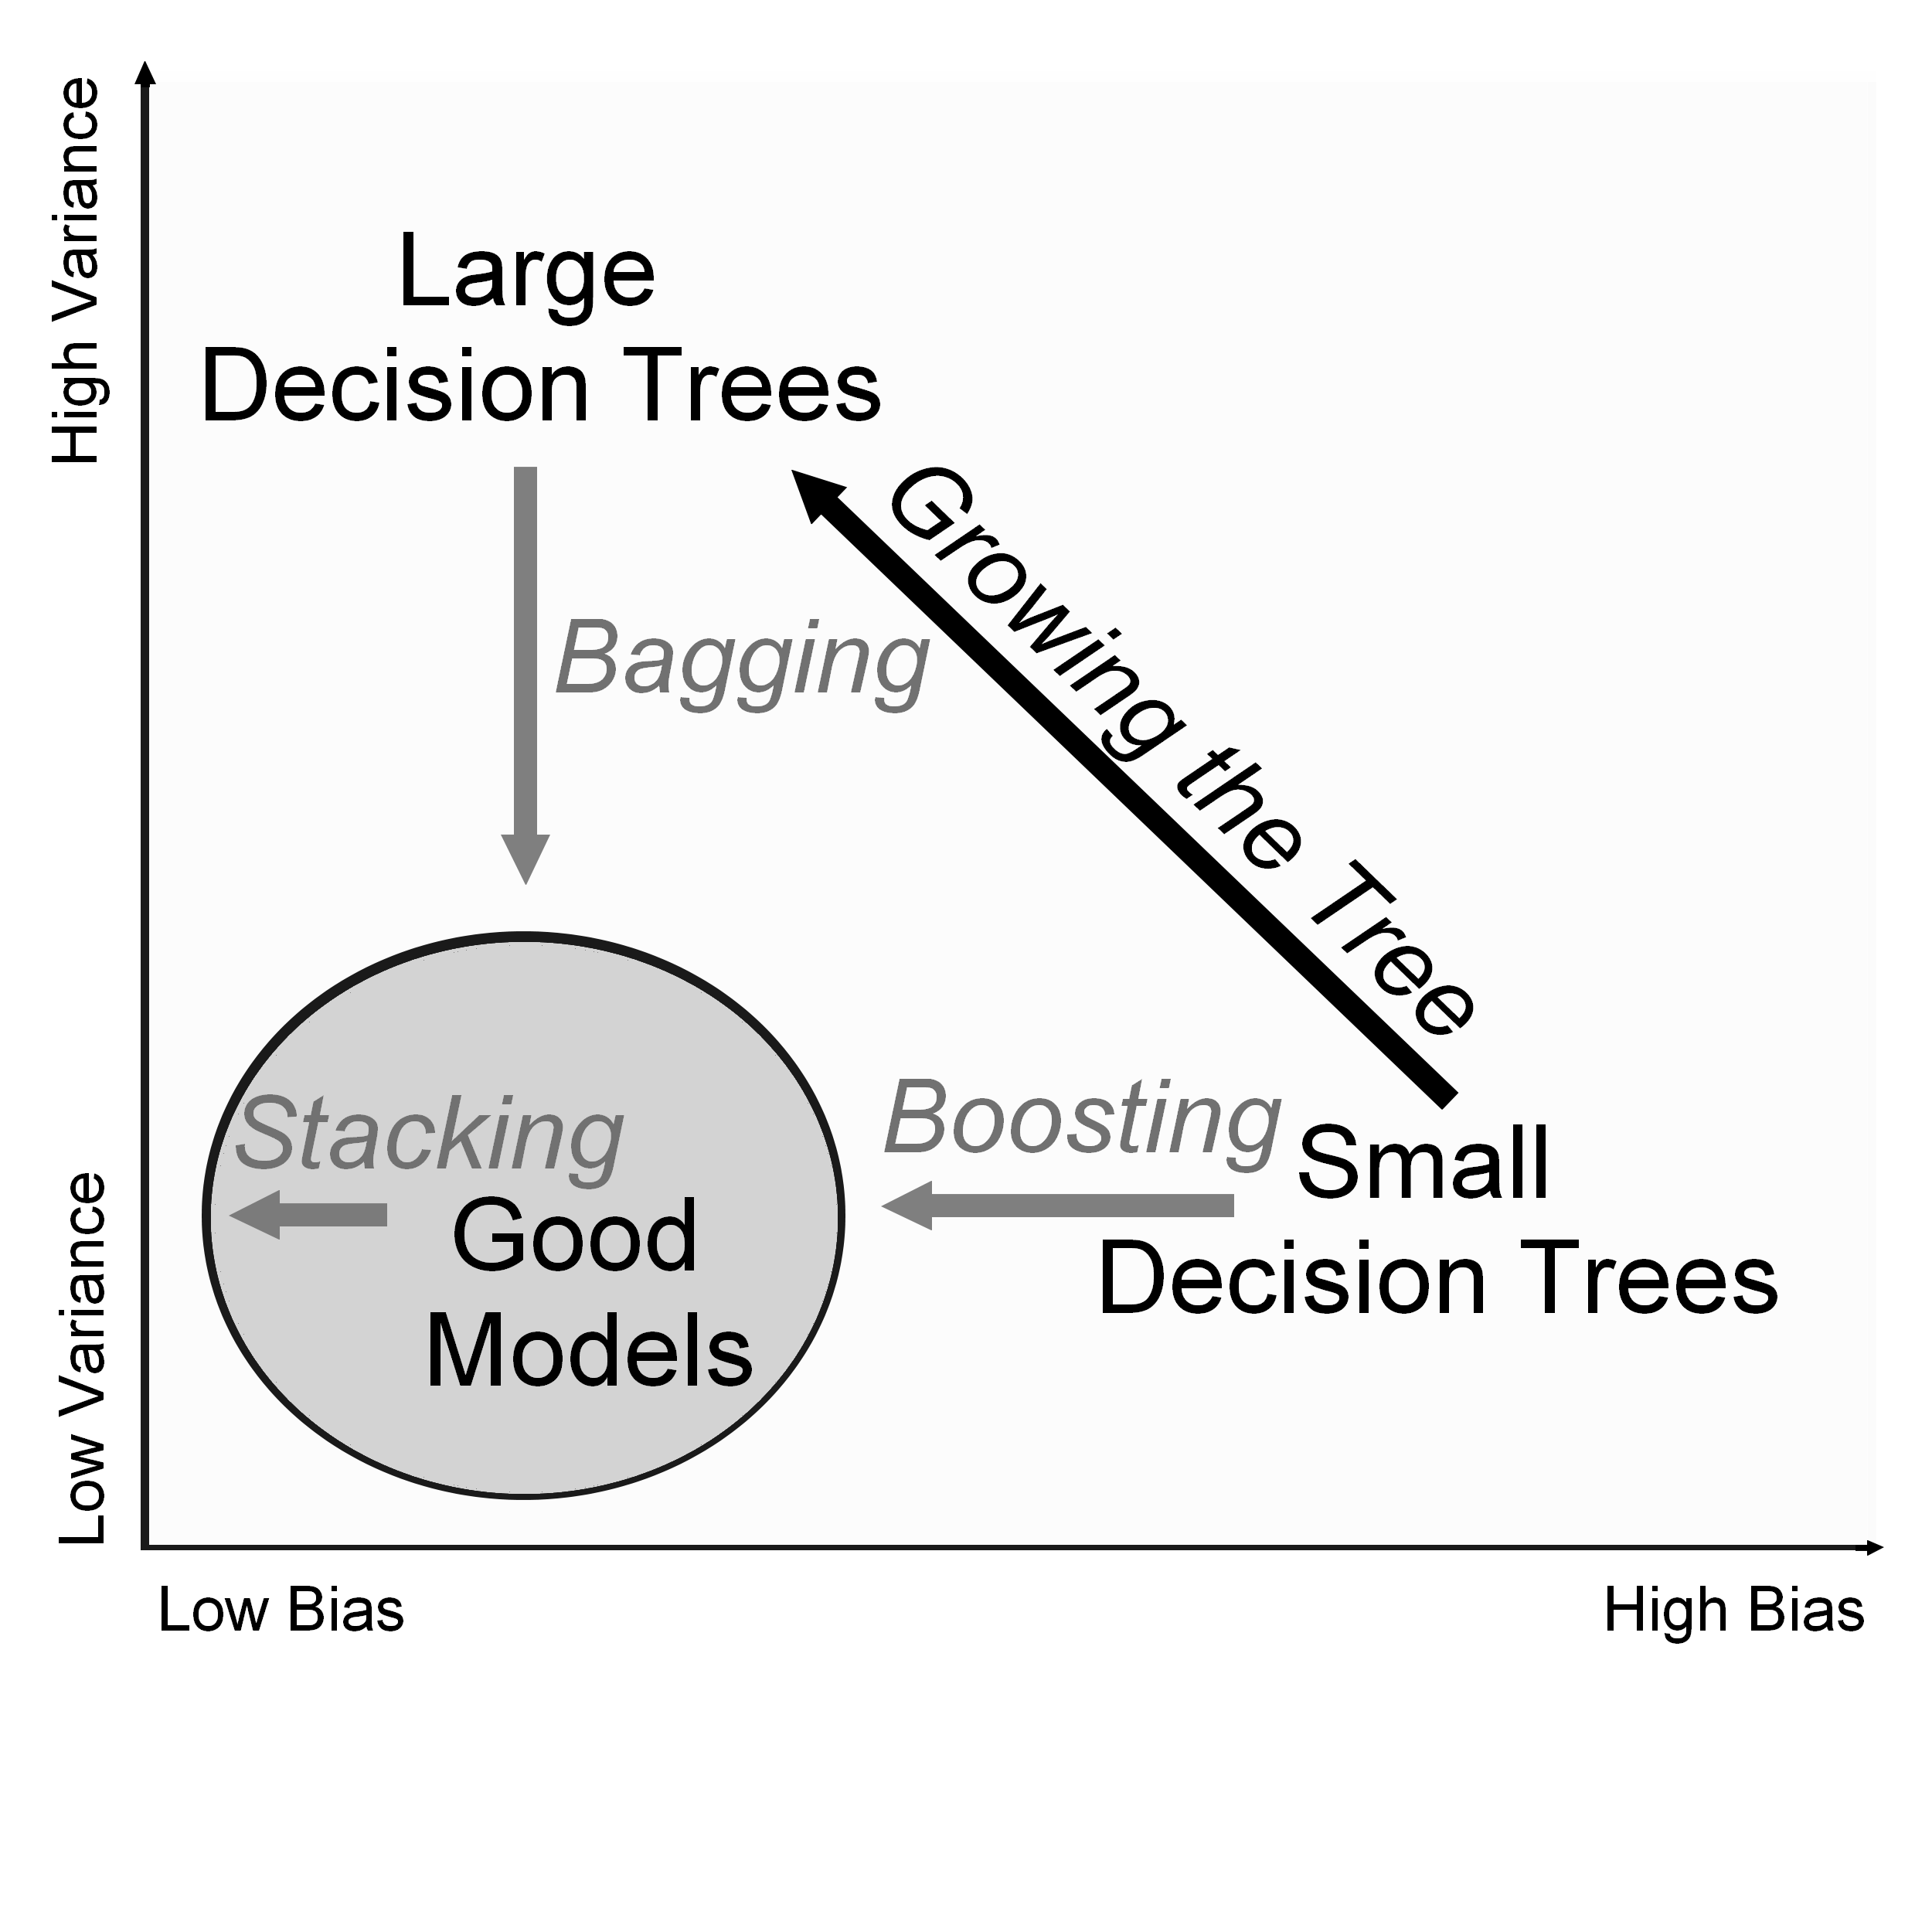
\includegraphics[trim={0cm 4.5cm 0cm 1cm}, clip, scale=0.2]{graphs/biasvariance_reduction_bw.png}}
\caption[Bias and Variance Reduction]{Reduction of Bias and Variance by Stacking and Ensembling methods with Decision Trees as base learners.}\label{bv}
\end{figure} 


\section{Credit Risk Assessment}
Techniques of Stacking and Ensemble modelling are applied to predictive problems of a broad range of topics. This paper will especially focus on the application of Ensemble Learning in credit risk classification problems. Credit risk assessment and especially its modelling is an important part in the field of financial risk management since for most small- and medium-sized banks, interests on loans are still the primary financial source \citep[p.2]{jacobson2006internal}. The banking supervision accord Basel II, that was published in 2004 and applies to member states of the European Union since 2007, restricted the buffer capital on banks and therefore makes it especially important for them to estimate the riskiness of loan applicants \citep{basel2}. For that, banks need to be able to distinguish between risky and non-risky applicants. Two opposing factors determine the banks' business rules regarding loans: On the one hand, more loans are better for the bank. On the other hand, a bank can not afford to make to many bad decisions, since this would eventually lead to a collapse of the bank. A good strategy on granting loans will therefore be a compromise. Minimizing the fraction of bad decisions thus increases banks' revenue.

Applying Ensemble Learning techniques to credit risk modelling has already proven to be highly valuable. Zhu et al. (\citeyear{zhu2017comparison}) investigate credit risk assessment for small- and medium-sized Chinese enterprises. For that, they carry out an experiment in which they compare the predictive performance of individual machine learning methods and Ensembling methods of different complexity. They find especially the more complex ensembling methods to be of outstanding discriminative accuracy \citep[p.46f.]{zhu2017comparison}. Yu et al. (\citeyear{yu2008credit}) successfully apply an Ensemble learner comprising six levels of stacked Neural Networks in order to evaluate credit risk at the measurement level. Hereby, they further incorporate the Bagging approach. They conclude, that such technique "provides a promising solution to credit risk analysis" \citep[p.1443]{yu2008credit}. 




\section{Methodology}
In order to evaluate and compare the introduced Stacking and Ensemble models, an empirical evaluation study is conducted. The quantlets for replication of the study can be found in the Appendix \ref{code} or accessed in the corresponding \href{https://github.com/schreckf/NIC_Schreck}{\color{black}{github repository}}. In this section, the dataset used for the evaluation study is presented, the model building process is explained in detail and the metrics for evaluation are introduced.

\subsection{Data description}
The empirical evaluation study of this paper uses the German Credit Dataset from the UCI machine learning repository \citep{dataset}. This dataset classifies people as either being good or bad customers for a bank with respect to credit risk. It comprises a total number of 1000 observations and 20 features. Tables \ref{summary_numeric} and \ref{summary_categorical} in the Appendix present the summary statistics for the numerical and the categorical features in the original dataset, respectively. To ensure better model performance, the numerical data is standardized before model building. The dataset is partitioned into a training dataset, comprising 750 observations, and into a test dataset, comprising 250 observations.





\subsection{Model building process}
The model building process consists of feature selection, model training and tuning as well as prediction. For the purpose of this study, an extensive set of models went through this process: a Random Forest model and a Gradient Boosting model represent the Ensemble learners. Furthermore, both models are built a second time as level 0 generalizers for the Stacked Generalization models. Additionally, a Decision Tree, a Neural Network as well as a Logistic Regression model are built in order to provide a diverse set of level 0 generalizers for the Stacking. Four different such Stacked Generalization models are built by using different subsets of base learners' predictions and different combiner algorithms. 

Before training the models, feature selection is a critical step. The aim of feature selection is dimension reduction. Building the models on an optimal subset of features may reduce their training time, reduce the variance and may make the model more easily interpretable \citep{guyon2003introduction}. Since, the optimal subset of features depends on each model, a wrapper approach for feature selection is applied to each model specifically. Each model-specific wrapper approach starts with building an intercept model and sequentially adding the next best feature by using a sequential foreward selection approach. The wrapper approach stops when adding another feature cannot increase the AUC measure (see section \ref{metrics}) by at least $0.00001$ units. All wrapper approaches are run on 3-fold cross-validation in order to avoid overfitting problems. Notably, a larger number of folds leads to instabilities due to the small sample size. Subsequently, the subset of features identified by the model-specific wrapper approaches is used for training of the corresponding models. Since the Random Forest and the Gradient Boosting models are built as Ensemble models as well as level 0 generalizers for the Stacked Generalization models, independent wrapper approaches are applied for both versions.

The training process for each model generally consists of establishing a broad-grid tuning of all relevant hyperparameters on the training dataset in order to find the (locally) optimal parameter choices. In order to avoid overfitting on the training dataset, each combination of hyperparameters is tested by a 3-fold cross-validation process. For the Random Forest and the Gradient Boosting model, their tuned versions can directly be used for prediction on the test dataset. For the Stacked Generalization models, the training dataset is partitioned into five disjoint subsets. Each of the five level 0 generalizers is then build in five iterations as described in section \ref{stacking}. Again, each iteration involves a parameter tuning on 3-fold cross-validation. All level 0 generalizers are then used to predict the observations in the test dataset. Stacking model 1 is then built by averaging over the probabilistic predictions of all five level 0 generalizers. Stacking model 2 is constructed by averaging over the probabilistic predictions of the three best predictions of level 0 generalizers in terms of AUC measure. For that, the correlations of the level 0 generalizers on the training data must be investigated in order to avoid multicollinearity problems. Stacking model 3 is built by using again all level 0 predictions and a Gradient Boosting model as combining algorithm. Finally, Stacking model 4 is constructed by combining all level 0 predictions by using a Logistic Regression combiner. The parameters of the combining algorithms are again tuned under 3-fold cross-validation.

\subsection{Evaluation metrics}\label{metrics}
In credit risk modelling, the misclassification costs are often type-specific. This means that a false negative prediction may have different costs for the bank than a false positive prediction. When misclassification costs are known, a cost-sensitive model building strategy should be consulted. Since in the context of this paper misclassification costs are however unknown, equal misclassification costs for false negative and false positive predictions are assumed. Furthermore, the broad field of cost-sensitive learning may serve as a topic for other studies. The following metrics are used to evaluate the models.

\paragraph{AUC:} In the model building process, tuning of model parameters for each model $m$ is evaluated on the Area Under Curve (AUC) metric. Tuning on the AUC is especially recommended when facing probabilistic predictions, since the metric generalizes over all possible cut-off thresholds that could be used to transform probabilistic into binary predictions. The AUC is a ranking indicator that measures the area under the receiver operating characteristic curve (ROC curve) \citep{hanley1982meaning}. For a probabilistic prediction, like in the context of this study, a visualization of the ROC curve can be obtained by plotting the sensitivity against $1 -$ specificity for all cut-off thresholds between zero and one. The AUC value can therefore take values between zero and one as well. A random model would obtain an AUC value of $0.5$, which can thus function as a benchmark value in model evaluation on AUC. In a statistical sense, the AUC estimates the probability that a randomly chosen correct prediction is correctly ranked higher than a randomly chosen false prediction. For model $m$, the AUC can be calculated as
\begin{equation}
\text{AUC}^m = \frac{1}{P \times N}\sum_{j=1}^{P}\sum_{k=1}^{N}(\hat{y}^m_j - \hat{y}^m_k)
\end{equation}
, whereby $P$ and $N$ denote the positive (in our case \textit{good}) and negative (\textit{bad}) instances amongst the outcome values in the credit data. Further, $\hat{y}^m_j$ and $\hat{y}^m_k$ are the predictions of model $m$ for the positive instance $y_j$ and the prediction for the negative instance $y_k$, respectively.

\paragraph{Accuracy:} Another important metric in evaluation of classification models is the Accuracy metric, which can be interpreted as the percentage of correctly classified points. In contrast to the AUC, probabilistic predictions must be transformed into binary predictions for the Accuracy metric, which implies selecting a cut-off threshold. For the purpose of this study, a natural cut-off threshold of $0.5$ is chosen.
\begin{equation}
\text{Accuracy}^m = \frac{TP^m + TN^m}{FP^m + FN^m + TP^m + TN^m}
\end{equation}
, whereby $TP^m$ is the number of true positive predictions for model $m$ and $TN^m$, $FP^m$ and $FN^m$ are the corresponding number of true negatives, the number of false positives and the number of false negatives for model $m$, respectively.

\paragraph{Logarithmic Loss:} The Logarithmic Loss is a metric for evaluating class predictions that penalizes for a high confidence about incorrect classifications. For the case of a binary outcome, the Logarithmic Loss is given by\\
\begin{equation}
\text{LogLoss}^m = - \frac{1}{N}\sum_{i=1}^{N}(y_i\times\log(p^m_i) + (1 - y_i)\times\log(1 - p^m_i))
\end{equation}
, whereby $p^m_i$ is model $m$'s prediction for observation $y_i$.

\paragraph{Brier Score:} The models will further be assessed on the Brier Score, which is identical to the Mean Squared Error metric in statistics. For model $m$, the Brier score is defined as 
\begin{equation}
\text{Brier}^m = \frac{1}{N}\sum_{i=1}^{N}(y_i - \hat{y}^m_i)^2
\end{equation}
, whereby $\hat{y}^m_i$ denotes the predicted probability of model $m$ for observation $y_i$. 


\section{Results}\label{results}
In the following, the results of the empirical application of Stacking and Ensemble models on a credit risk classification problem will be presented. Table \ref{eval} shows the evaluations of all models on the test dataset with respect to the metrics AUC, Accuracy, Logarithmic Loss and Brier Score. 

\begin{table}[ht]
\centering
\begin{tabular}{lrrrr}
  \hline
 Model category: Model & AUC & Accuracy & LogLoss & Brier\\ 
  \hline
Ensemble model: Random Forest & 0.78 & 0.73 & 0.52 & 0.18 \\ 
Ensemble model: Gradient Boosting & 0.78 & 0.72 & 0.52 & 0.18 \\
\hline 
  Level 0 generalizer: Decision Tree & 0.69 & 0.65 & 0.60 & 0.21 \\ 
  Level 0 generalizer: Logit Regression & 0.71 & 0.74 & 0.57 & 0.19 \\ 
  Level 0 generalizer: Neural Network & 0.76 & 0.74 & 0.53 & 0.18 \\ 
  Level 0 generalizer: Random Forest & 0.73 & 0.69 & 0.56 & 0.19 \\ 
  Level 0 generalizer: Gradient Boosting & 0.80 & 0.74 & 0.52 & 0.17 \\ 
\hline
  Stacking model 1: Average, all predictions & 0.77 & 0.64 & 0.24 & 0.18 \\ 
  Stacking model 2 Average, best predictions & 0.77 & 0.63 & 0.25 & 0.18 \\ 
  Stacking model 3: GB, all predictions & 0.78 & 0.61 & 0.29 & 0.17 \\ 
  Stacking model 4: LR, all predictions & 0.81 & 0.64 & 0.30 & 0.16 \\ 
   \hline
\end{tabular}
\caption[Model performances on the test dataset]{Model performances on the test dataset. Values rounded on two digits after comma. Abbreviations GB and LR denote Gradient Boosting and Logistic Regression that are used as combiner algorithms.}\label{eval}
\end{table}

\noindent Since all models were tuned on the AUC metric, the comparison on behalf of this metric is most informative. The two Ensemble models, namely the Random Forest and the Gradient Boosting model, score highly on the AUC metric with a value of $0.78$. In terms of AUC, they even outperform most level 0 generalizers, especially the Decision Tree and the Logistic Regression. It can be concluded that they rank a randomly chosen correct prediction comparatively comparatively higher than a randomly chosen false prediction in comparison with the level 0 generalizers. Notably, the Gradient Boosting level 0 generalizer and the Random Forest level 0 generalizer perform a bit different when compared to their counterparts. This may origin from the decreased size of training dataset due to the partitioning that was applied for building the level 0 generalizers. 

\noindent The four Stacking models were built on top of the level 0 generalizers. Figure \ref{corrgram} shows the correlations of the predictions of the level 0 generalizers on the training data. It can be seen that the predictions of the level 0 generalizers are (mostly) correlated positively, which seems intuitive since they all predict the target in the similar context. However, correlations are not perfect (all $<|0.9|$). This reveals diversity of predictions, which already indicates that combining them may increase predictive performance.

\begin{figure}[htp] \centering{
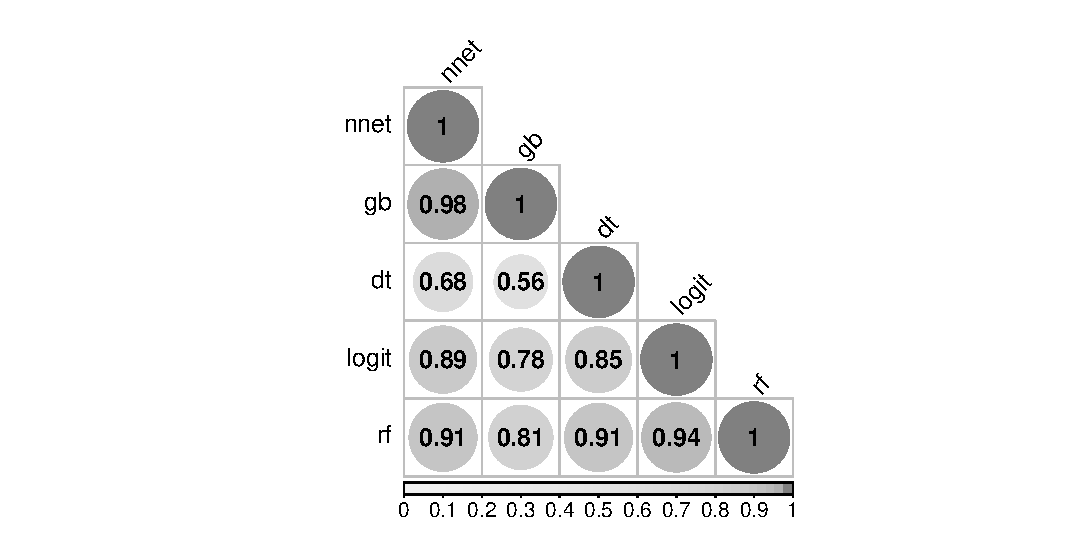
\includegraphics[trim={1cm 3.2cm 1cm 2cm}, clip, scale=0.74]{graphs/corrgram.pdf}}
\caption[Correlation of predictions]{Correlation plot of training dataset predictions of level 0 generalizers.}\label{corrgram}
\end{figure}  

Indeed, Table \ref{eval} reveals that the four Stacking models clearly outperform their level 0 generalizers in terms of AUC. Stacking models 1, 2 and 3 that are based on averaging predictions as well as a Gradient Boosting combiner have similar high AUC performance than the Random Forest and the Gradient Boosting model. Stacking model 4 that is based on combining level 0 predictions by Logistic Regression even shows a better AUC performance than the Random Forest and the Gradient Boosting model. For visual comparison, Figure \ref{aucplot} shows the ROC curves related to the AUC values for all models.

\begin{figure}[!htp] \centering{
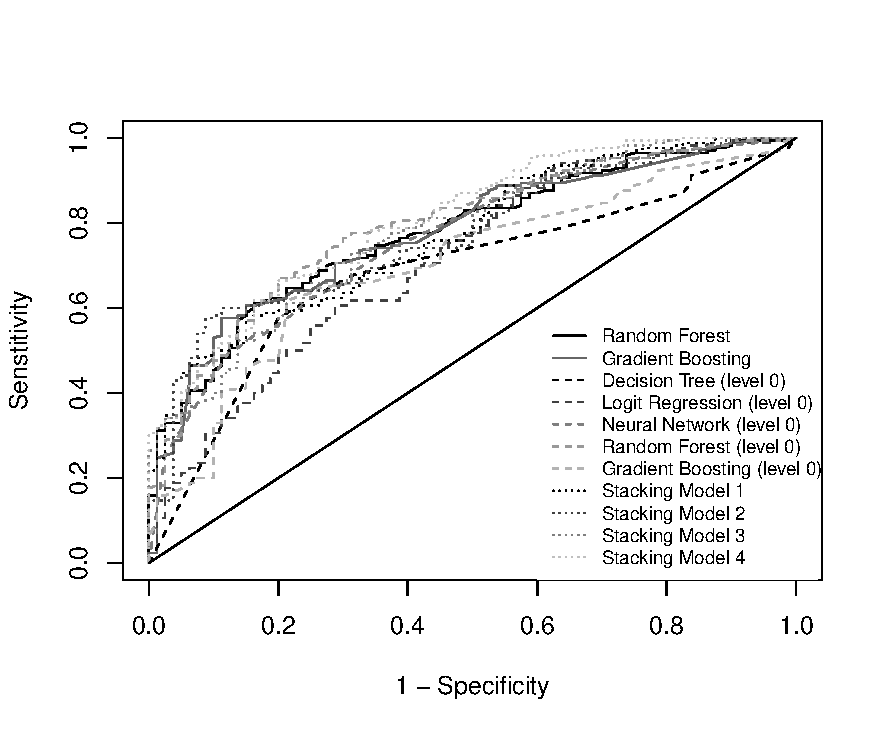
\includegraphics[trim={0cm 0.5cm 0cm 1.8cm},clip, scale=0.85]{graphs/auplot_final.pdf}}
\caption[ROC curves]{Receiver Operating Characteristic (ROC) curves for the predictions of all models. The diagonal line represents the ROC curve of a random model.}\label{aucplot}
\end{figure} 


With regards to the Accuracy, the Logistic Regression and the Neural Network perform about equally well as the two Ensemble models. The Decision Tree is however outperformed by the Random Forest and the Gradient Boosting model. Interestingly, all four Stacking models show relatively bad values on the Accuracy metric. Regarding the relation of Accuracy and AUC, it can be concluded that the Stacking and Ensemble models do not necessarily perform better on the cut-off threshold of $0.5$, which is implied by the Accuracy metric. However, generalizing over all possible cut-off threshold they clearly outperform most level 0 generalizers as can be seen by the corresponding AUC values. Deeper insights can be obtained by the corresponding ROC curves in Figure \ref{aucplot}, which gives an impression on the models' relative performances. ...
Furthermore, this indicates that the standard cut-off threshold for probabilistic predictions of $0.5$ may not be optimal for those models.

The Logarithmic Loss metric gives even more information on the particular strengths and weaknesses of the models. Contrasting the level 0 generalizers with the Random Forest and the Gradient Boosting model, the latter show a slightly smaller Logarithmic Loss. The four Stacking models however, reveal a much better performance on behalf of the Logarithmic Loss metric. It can be concluded, that the Ensemble models and even more the Stacking models do not place as high confidences on their incorrect predictions. 

Regarding the Brier Score, differences are not that present. In tendency, the Stacking and Ensemble Models perform slightly better on that metric than the level 0 generalizers. One time more, this shows that in binary classification a good model is not only defined by its errors but rather by which observations it is able to classify correctly.

With regards to all calculated metrics, Stacking models are be able to capture the structure in the data most effective. Already a simple averaging approach, as applied for Stacking models 1 and 2, leads to increased performance when compared to the level 0 models. Interestingly, reducing the set of level 0 generalizers, like for Stacking model 2, does not add more value. Nevertheless, it shall be noted that such restriction of input predictions could still decrease computational costs. Applying a more sophisticated level 1 combiner, like Gradient Boosting or Logistic Regression, furthermore improves prediction. In particular, the Logistic Regression combiner is able to increase AUC performance. 


\newpage
\section{Conclusion}
This paper aimed to discuss and evaluate Stacking and Ensemble models in a financial application of credit risk assessment. Focus was set on introducing the concepts of Bagging, Boosting and Stacked Generalization as well as the corresponding Random Forest and Gradient Boosting models. In depth, it was explained how Bagging and Boosting aim at increasing performance by decreasing generalization variance of base learners and by decreasing generalization bias of base learners, respectively. Moreover, the Stacked Generalization model was outlined, that seeks for the optimal way to combine the specific strengths of level 0 generalizers in order to increase predictive performance even more.

A broad set of different Stacking and Ensemble models as well as standard machine learning models was applied and evaluated to a classification problem of credit risk assessment. Thereby, the Random Forest model and Gradient Boosting model outperformed standard machine learning models on behalf of the calculated metrics. Furthermore, all four Stacked Generalization approaches were able to establish a better performance on AUC, Logarithmic Loss and Brier Score than their level 0 generalizers. With regards to Accuracy metric, they performed worse, suggesting that the metric-implied cut-off threshold of $0.5$ being suboptimal. Even a simple combiner algorithm like averaging could increase performance of the Stacking model, while the Logistic Regression combiner performed best. Restricting the subset of input predictions seems to be ineffective with regards to performance issues. To conclude, Stacking and Ensemble models could show their comparative strengths in this study. The results strongly confirm their value for prediction issues in credit risk assessment.

While this study focused on predicting binary outcomes, further research could evaluate the performance of Stacking and Ensemble models for regression problems in a similar context. A shortfall of Stacking and Ensemble models is their need of much computational resources caused by their complexity. In the context of \textit{scalability}, current research tests ideas that restrict computational costs, e.g. by adaptive parallelization \citep{li2014communication} or by improving intra-model algorithms like stochastic gradient descent \citep{bottou2012stochastic}. A further problem of such models is the absence of proven statistical properties like unbiasedness, consistency or asymptotic theory for construction of confidence intervals. In order to use machine learning models for research purposes, such properties are however necessary. Only recently, the field of \textit{machine learning in economics} emerged, where the development of such properties is aimed at (see \cite{athey2017impact}, \citeauthor{wager2018est} \hyperlink{wager2018est}{(\color{Black}{in press})}). Developments in this field of research will also enable better application of machine learning models to financial research problems.







%----------------------------------------------------------------------------------------
%	APPENDIX
%----------------------------------------------------------------------------------------
\newpage
\appendix
\section{Appendix - Summary Tables}

\begin{table}[ht]
\centering
\begin{tabular}{lrrrrr}
  \hline
 Feature & Mean & Std. Dev. & Median & Minimum & Maximum \\ 
  \hline
Duration & 20.90 & 12.06 & 18.00 & 4.00 & 72.00 \\ 
  Amount & 3271.26 & 2822.74 & 2319.50 & 250.00 & 18424.00 \\ 
  Installment Rate & 2.97 & 1.12 & 3.00 & 1.00 & 4.00 \\ 
  Residence Duration & 2.85 & 1.10 & 3.00 & 1.00 & 4.00 \\ 
  Age & 35.55 & 11.38 & 33.00 & 19.00 & 75.00 \\ 
  Number of Credits & 1.41 & 0.58 & 1.00 & 1.00 & 4.00 \\ 
  Number of Liable People & 1.16 & 0.36 & 1.00 & 1.00 & 2.00 \\ 
   \hline
\end{tabular}
\caption[Summary statistics for numerical features]{Summary statistics for numerical features in the German Credit Dataset.}\label{summary_numeric}
\end{table}

\begin{table}[!ht]
\centering
\begin{tabular}{lllll}
  \hline
Feature & Category & Count & Fraction \\ 
  \hline
Customer Classification & good & 700 & 70\% \\ 
(Outcome Feature) &bad & 300 & 30\% \\
\hline
Account Status & x < 0 DM (D-Mark) & 274 & 27.4\% \\ 
 & 0 DM < x < 200 DM & 269 & 26.9\% \\ 
 & x >= 200 DM & 63 & 6.3\% \\ 
& no account & 394 & 39.4\% \\ 
\hline
Credit History & no credits taken/all paid back duly & 40 & 4\% \\ 
& all credits at this bank paid back duly & 49 & 4.9\% \\ 
 & existing credits paid back duly till now & 530 & 53\% \\ 
 & delay in paying off in the past & 88 & 8.8\% \\ 
 & critical account & 293 & 29.3\% \\ 
\hline
 Purpose & car (new) & 234 & 23.4\% \\ 
 & car(used & 103 & 10.3\% \\ 
&furniture/equipment & 12 & 1.2\% \\ 
&radio/television & 181 & 18.1\% \\ 
& domestic appliances & 280 & 28\% \\ 
 &repairs & 12 & 1.2\% \\ 
 &education & 22 & 2.2\% \\ 
 &vacation & 50 & 5\% \\ 
 &retraining & 9 & 0.9\% \\ 
 &business & 97 & 9.7\% \\ 
\hline
 Savings & x < 100 DM & 603 & 60.3\% \\ 
&100 <= x <  500 DM & 103 & 10.3\% \\ 
&500 <= x < 1000 DM & 63 & 6.3\% \\ 
&x >= 1000 DM & 48 & 4.8\% \\ 
&unknown/no savings & 183 & 18.3\% \\ 
\hline\\
(continued on next page) & & & 
\end{tabular}
\end{table}

\begin{table}[!ht]
\centering
\begin{tabular}{lllll}
 (continued)& & &\\ \\
\hline
Feature & Category & Count & Fraction \\ 
  \hline
 Employment Duration & unemployed & 62 & 6.2\% \\ 
&x < 1 year & 172 & 17.2\% \\ 
&1  <= x < 4 years & 339 & 33.9\% \\ 
&4  <= x < 7 years & 174 & 17.4\% \\ 
&x >= 7 years & 253 & 25.3\% \\ 
\hline
Status and Sex & male: divorced/separated & 50 & 5\% \\ 
&female: divorced/separated/married & 310 & 31\% \\ 
&male: single & 548 & 54.8\% \\ 
&male: married/widowed & 92 & 9.2\% \\ 
\hline
 Other Debtors & none & 907 & 90.7\% \\ 
&co-applicant & 41 & 4.1\% \\ 
&guarantor & 52 & 5.2\% \\ 
\hline
  Property & real estate & 282 & 28.2\% \\ 
&savings agreement/life insurance & 232 & 23.2\% \\ 
&car or other& 332 & 33.2\% \\ 
&unknown/no property & 154 & 15.4\% \\ 
\hline
 Other Installment Plans & bank & 139 & 13.9\% \\ 
&stores & 47 & 4.7\% \\ 
&none & 814 & 81.4\% \\ 
\hline
Housing & rent & 179 & 17.9\% \\ 
&own & 713 & 71.3\% \\ 
&for free & 108 & 10.8\% \\ 
\hline
 Job & unemployed/ unskilled  - non-resident & 22 & 2.2\% \\ 
 & unskilled - resident & 200 & 20\% \\ 
 &skilled employee / official & 630 & 63\% \\ 
 &management/self-employed/officer & 148 & 14.8\% \\ 
 \hline
Telephone & none & 596 & 59.6\% \\ 
&yes & 404 & 40.4\% \\ 
 \hline
Foreign Worker & yes & 963 & 96.3\% \\ 
&no & 37 & 3.7\% \\ 
    \hline
\end{tabular}
\caption[Summary statistics for categorical features]{Summary statistics for categorical features in the German Credit Dataset.}\label{summary_categorical}
\end{table}


\clearpage

\section{Appendix - Code}\label{code}
\begin{algorithm}
\caption[Quantlet 1: Main file]{\href{https://github.com/schreckf/NIC_Schreck/blob/master/code}{\color{Black}\large\textbf{Main file}}}
\end{algorithm}

\begin{lstlisting}
###################################################################
# Numerical Introductory Course 2018
# Topic: Stacking and Ensemble Modelling
# Supervisor: Prof. Dr. Brenda López Cabrera
# Student: Frederik Schreck
###################################################################


#------------------------------------------------------------------
# Prepare environment
#------------------------------------------------------------------

# Install packages and set working directory to path of main.R file
library("rstudioapi")
setwd(dirname(rstudioapi::getActiveDocumentContext()$path))

library("plyr")
library("mlr")
library("parallelMap")
library("parallel")
library("ggplot2")
library("corrplot")
library("glmnet")
library("xtable")
library("caret")
library("caretEnsemble")
library("gbm")
library("ROCR")

rm(list = ls(all = TRUE))
graphics.off()


#------------------------------------------------------------------
# Loading dataset: German Credit Data
#------------------------------------------------------------------

creditdata           <- read.delim("dataset/german_credit_data.txt", 
                                   header = FALSE, sep = " ")

# Renaming of feature
colnames(creditdata) <- c("account_status", "duration", 
                           "credit_history", "purpose", "amount", 
                           "savings", "employment_duration", 
                           "installment_rate", "status_sex", 
                           "other_debtors", "residence_duration", 
                           "property", "age", "installment_plans", 
                           "housing", "number_credits", "job", 
                           "liable_people", "telephone", 
                           "foreign_worker", "customer")


#------------------------------------------------------------------
# Feature Engineering
#------------------------------------------------------------------

# Formatting and labelling
creditdata$duration           <- as.numeric(creditdata$duration)
creditdata$amount             <- as.numeric(creditdata$amount)
creditdata$installment_rate   <- as.numeric(creditdata$installment_rate)
creditdata$residence_duration <- as.numeric(creditdata$residence_duration)
creditdata$age                <- as.numeric(creditdata$age)
creditdata$number_credits     <- as.numeric(creditdata$number_credits)
creditdata$duration           <- as.numeric(creditdata$duration)
creditdata$liable_people      <- as.numeric(creditdata$liable_people)
creditdata$customer           <- factor(creditdata$customer, 
                                        levels = c(1, 2), 
                                        labels = c("good", "bad"))

# No problem of missing values
apply(creditdata, 2, function(x) sum(is.na(x)))

# Create summary tables for numeric and for categorical features
numeric_vars <- lapply(Filter(is.numeric, creditdata), 
                       function(x) rbind(mean = mean(x),
                                         sd = sd(x),
                                         median = median(x),
                                         minimum = min(x),
                                         maximum = max(x)))
print(xtable(t(data.frame(numeric_vars))), 
      file="tables/summary_numeric.txt")


cat_vars <- ldply(Filter(is.factor, creditdata), 
                  function(x) t(rbind(names(table(x)),
                                      table(x),
                                      paste0(prop.table(table(x))*100,"%"))))
colnames(cat_vars) <- c("feature", "category", "Count", "Fraction")
print(xtable(data.frame(cat_vars)), 
      file="tables/summary_categorical.txt")

# Standardize numeric features for models performance
creditdata$duration           <- scale(creditdata$duration)
creditdata$amount             <- scale(creditdata$amount)
creditdata$installment_rate   <- scale(creditdata$installment_rate)
creditdata$residence_duration <- scale(creditdata$residence_duration)
creditdata$age                <- scale(creditdata$age)
creditdata$number_credits     <- scale(creditdata$number_credits)
creditdata$duration           <- scale(creditdata$duration)
creditdata$liable_people      <- scale(creditdata$liable_people)


#------------------------------------------------------------------
# Data partitioning into training and testing data
#------------------------------------------------------------------

set.seed(2601)
idx   <- sample(x = NROW(creditdata),
                size = floor(0.75*NROW(creditdata)), 
                replace = FALSE)
train <- creditdata[idx,]
test  <- creditdata[-idx,]


#------------------------------------------------------------------
# Feature Selection
#------------------------------------------------------------------

'For each model, a wrapper approach is run on the training dataset 
in order to find the best subset of features. The optimal set of
features is the then used in the subsequent model building part. 

The wrappers as well as the model tuning are evaluated on the AUC
measure. Tuning of the hyperparameters in the wrapper is done by 
a grid-approach with 3-fold cross-validation process. 

For reproduction of the results, the output of the wrapper 
files can be accessed directly.'

# Generate empty lists to store the models and their results in
vars       <- list() # Selected set of features used for each model
model_lib  <- list() # Model library
yhat       <- list() # Predictions on test dataset


##### Gradient Boosting wrapper ###################################
source("gb_wrapper.R")

# For replication purposes: gb_wrapper results
train_wrapper <- mlr::createDummyFeatures(train, target = "customer")
vars$gb       <- c("customer", "account_status.A11", 
                   "account_status.A14", "credit_history.A30",
                   "credit_history.A34", "purpose.A49", "savings.A63",
                   "savings.A65", "employment_duration.A75",
                   "other_debtors.A103", "property.A123",
                   "installment_plans.A143", "job.A174",
                   "telephone.A192")       


##### Random forest wrapper #######################################
source("rf_wrapper.R")

# For replication purposes: rf_wrapper results
vars$rf      <- c("customer", "account_status", "duration", 
                  "credit_history", "purpose", "savings",
                  "employment_duration", "other_debtors",
                  "residence_duration", "age", "installment_plans",
                  "housing", "job", "liable_people", "foreign_worker")


##### Stacked Generalization model ################################
'For the Stacked Generalization model, firstly the training data is
split into five disjoint sets. Secondly, the Random Forest model and 
the Gradient Boosting model are rebuilt on that subset. For each 
model, a new wrapper approach is applied to find the optimal subset
of features.

Additionally, a Decision Tree, a Logistic Regression and a 
Neural Network are built. Similar to the models before, a 
model-specific wrapper approach is applied before the model
building process.

For reproduction of the results, the output of the wrapper 
functions can again be accessed directly.
'

##### Stacking: Decision tree wrapper #############################
source("dt_wrapper.R")

# For replication purposes: dt_wrapper results
vars$dt       <- c("customer", "account_status", "credit_history",
                   "savings", "number_credits")

##### Stacking: Logit wrapper #####################################
source("logit_wrapper.R")

# For replication purposes: logit_wrapper results
vars$logit    <- c("customer", "duration", "credit_history",
                   "purpose", "amount", "installment_rate",
                   "status_sex", "residence_duration", "age",
                   "installment_plans", "number_credits",
                   "liable_people", "telephone", "foreign_worker")  

##### Stacking: Neural net wrapper ################################
source("nnet_wrapper.R")

# For replication purposes: nnet_wrapper results
vars$nnet     <- c("customer", "account_status", "credit_history")

##### Stacking: Gradient Boosting wrapper #########################
source("gb_wrapper_stacking.R") 

# For replication purposes: gb_wrapper results
vars$gb2      <- c("customer", "account_status.A11", 
                   "account_status.A14", "credit_history.A34",
                   "purpose.A41", "savings.A65", 
                   "employment_duration.A74", "status_sex.A94",
                   "other_debtors.A103", "installment_plans.A143")      

##### Stacking: Random forest wrapper #############################
source("rf_wrapper_stacking.R")

# For replication purposes: rf_wrapper results
vars$rf2      <- c("customer", "account_status", "duration",
                   "credit_history", "purpose", "savings",
                   "employment_duration", "other_debtors",
                   "residence_duration", "age",
                   "installment_plans", "housing", "job",
                   "liable_people", "foreign_worker")


#------------------------------------------------------------------
# Model Building
#------------------------------------------------------------------

'In the following, the models are built, parameters are tuned and 
predictions on the test dataset are made. Each model uses the 
optimal subset of features from  the corresponding wrapper approach.'

###### Random forest tuning #######################################
source("rf_model.R")


###### Gradient Boosting tuning ###################################
source("gb_model.R")


###### Stacking: preparation ######################################

# Partitioning the dataset for the Stacking into five equally 
# sized disjoint sets
set.seed(2610)
idx2       <- sample(rep(1:5,each = nrow(train)/5)) 
train_sets <- lapply(split(1:nrow(train), idx2), 
                     function(i) creditdata[i,])

###### Stacking: Decision tree tuning #############################
source("dt_model.R")


###### Stacking: Logit model ######################################
# No tuning necessary 
source("logit_model.R")


###### Stacking: Neural net tuning ################################
source("nnet_model.R")


###### Stacking: Gradient Boosting tuning #########################
source("gb_model_stacking.R")


###### Stacking: Random forest tuning #############################
source("rf_model_stacking.R")


###### Stacked Generalization Models ##############################
source("st_model.R")


#------------------------------------------------------------------
# Model evaluation
#------------------------------------------------------------------

'After having built all the models, they can now be compared and 
evaluated with regard to a variety of evaluation metrics.'

# Create empty lists to store the measure values in
auc        <- list() # Area under curve performance measure
acc        <- list() # Accuracy performance measure
kappa      <- list() # Kappa performance measure
logloss    <- list() # Logarithmic Loss measure
brier      <- list() # Brier score measure 

# AUC
auc$rf     <- mlr::performance(yhat$rf, 
                               measures = mlr::auc); auc$rf
auc$gb     <- mlr::performance(yhat$gb, 
                               measures = mlr::auc); auc$gb
auc$dt     <- mlr::performance(yhat$dt_test, 
                               measures = mlr::auc); auc$dt
auc$logit  <- mlr::performance(yhat$logit_test, 
                               measures = mlr::auc); auc$logit
auc$nnet   <- mlr::performance(yhat$nnet_test, 
                               measures = mlr::auc); auc$nnet
auc$gb2    <- mlr::performance(yhat$gb2_test, 
                               measures = mlr::auc); auc$gb2
auc$rf2    <- mlr::performance(yhat$rf2_test, 
                               measures = mlr::auc); auc$rf2
auc$st1    <- measureAUC(probabilities = yhat$st1$prob.good, 
                      truth = yhat$st1$truth, positive = "1", 
                      negative = "2"); auc$st1
auc$st2    <- measureAUC(probabilities = yhat$st2$prob.good, 
                      truth = yhat$st2$truth, positive = "1", 
                      negative = "2"); auc$st2
auc$st3    <- measureAUC(probabilities = yhat$st3[,3], 
                         truth = yhat$st3[,2], positive = "1", 
                         negative = "2"); auc$st3
auc$st4    <- measureAUC(probabilities = yhat$st4[,3], 
                         truth = yhat$st4[,2], positive = "1", 
                         negative = "2"); auc$st4

# Accuracy
acc$rf     <- mlr::performance(yhat$rf, 
                               measures = mlr::acc); acc$rf
acc$gb     <- mlr::performance(yhat$gb, 
                               measures = mlr::acc); acc$gb
acc$dt     <- mlr::performance(yhat$dt_test, 
                               measures = mlr::acc); acc$dt
acc$logit  <- mlr::performance(yhat$logit_test, 
                               measures = mlr::acc); acc$logit
acc$nnet   <- mlr::performance(yhat$nnet_test,
                               measures = mlr::acc); acc$nnet
acc$gb2    <- mlr::performance(yhat$gb2_test,
                               measures = mlr::acc); acc$gb2
acc$rf2    <- mlr::performance(yhat$rf2_test, 
                               measures = mlr::acc); acc$rf2
acc$st1    <- measureACC(response = round(yhat$st1$prob.good), 
                         truth = yhat$st1$truth); acc$st1
acc$st2    <- measureACC(response = round(yhat$st2$prob.good), 
                         truth = yhat$st2$truth); acc$st2
acc$st3    <- measureACC(response = round(yhat$st3[,3]), 
                         truth = yhat$st3[,2]); acc$st3
acc$st4    <- measureACC(response = round(yhat$st4[,3]), 
                         truth = yhat$st4[,2]); acc$st4

# Logarithmic Loss
logloss$rf    <- mlr::performance(yhat$rf, 
                                  measures = mlr::logloss)
logloss$rf
logloss$gb    <- mlr::performance(yhat$gb, 
                                  measures = mlr::logloss)
logloss$gb
logloss$dt    <- mlr::performance(yhat$dt_test, 
                                  measures = mlr::logloss)
logloss$dt
logloss$logit <- mlr::performance(yhat$logit_test,
                                  measures = mlr::logloss)
logloss$logit
logloss$nnet  <- mlr::performance(yhat$nnet_test, 
                                  measures = mlr::logloss)
logloss$nnet
logloss$gb2   <- mlr::performance(yhat$gb2_test, 
                                  measures = mlr::logloss)
logloss$gb2
logloss$rf2   <- mlr::performance(yhat$rf2_test, 
                                  measures = mlr::logloss)
logloss$rf2
log_loss=function(actual, predicted)
{
  result=-1/length(actual)*
    (sum((actual*log(predicted)+
            (1-actual)*log(1-predicted))))
  return(result)
}
logloss$st1   <- log_loss(yhat$st1$truth, yhat$st1$prob.good)
logloss$st1
logloss$st2   <- log_loss(yhat$st2$truth, yhat$st2$prob.good)
logloss$st2
logloss$st3   <- log_loss(yhat$st3[,2], yhat$st3[,3])
logloss$st3
logloss$st4   <- log_loss(yhat$st4[,2], yhat$st4[,3])
logloss$st4

# MSE/Brier score
brier$rf      <- mlr::performance(yhat$rf, 
                                  measures = mlr::brier); brier$rf
brier$gb      <- mlr::performance(yhat$gb, 
                                  measures = mlr::brier); brier$gb
brier$dt      <- mlr::performance(yhat$dt_test, 
                                  measures = mlr::brier); brier$dt
brier$logit   <- mlr::performance(yhat$logit_test,
                                  measures = mlr::brier); brier$logit
brier$nnet    <- mlr::performance(yhat$nnet_test, 
                                  measures = mlr::brier); brier$nnet
brier$gb2     <- mlr::performance(yhat$gb2_test, 
                                  measures = mlr::brier); brier$gb2
brier$rf2     <- mlr::performance(yhat$rf2_test, 
                                  measures = mlr::brier); brier$rf2
brier$st1     <- measureBrier(probabilities = yhat$st1$prob.good, 
                              truth = yhat$st1$truth, 
                              positive = 1, negative = 2); brier$st1
brier$st2     <- measureBrier(probabilities = yhat$st2$prob.good, 
                              truth = yhat$st2$truth, positive = 1, 
                              negative = 2); brier$st2
brier$st3     <- measureBrier(probabilities = yhat$st3[,3], 
                              truth = yhat$st3[,2], positive =1, 
                              negative = 2); brier$st3
brier$st4     <- measureBrier(probabilities = yhat$st4[,3], 
                              truth = yhat$st4[,2], positive = 1, 
                              negative = 2); brier$st4

# Make evaluation table
eval_table           <- cbind(auc, acc, logloss, brier)
rownames(eval_table) <- c("Random Forest", "Gradient Boosting", 
                          "Decision Tree (level 0)", 
                          "Logit Regression (level 0)",
                          "Neural Network (level 0)", 
                          "Random Forest (level 0)", 
                          "Gradient Boosting (level 0)",
                          "Stacking Model 1", "Stacking Model 2", 
                          "Stacking Model 3", "Stacking Model 4")
colnames(eval_table) <- c("AUC", "Accuracy", 
                          "Logarithmic Loss", "Brier Score")


print(xtable(eval_table), file="tables/evaltable.txt")

# Generate plot with AUC curves for all models
plot(ROCR::performance(prediction(yhat$rf$data$prob.good, 
                            labels = matrix(test$customer, 
                                            nrow = NROW(test$customer), 
                                            ncol = 1))
                 , "tpr", "fpr"),
     colorize = FALSE, col = "gray0", type = "l",
     lty = 1, lwd = 1.2,
     xlab="1 - Specificity", ylab="Senstitivity")

plot(ROCR::performance(prediction(yhat$gb$data$prob.good, 
                            labels = matrix(test$customer, 
                                            nrow = NROW(test$customer), 
                                            ncol = 1))
                 , "tpr", "fpr"),
     colorize = FALSE, add = TRUE, col = "gray40",
     type = "l", lty = 1, lwd = 1.2)

plot(ROCR::performance(prediction(yhat$dt_test$data$prob.good, 
                            labels = matrix(test$customer, 
                                            nrow = NROW(test$customer), 
                                            ncol = 1))
                 , "tpr", "fpr"),
     colorize = FALSE, add = TRUE, col = "gray0",
     type = "l", lty = 2, lwd = 1.2)

plot(ROCR::performance(prediction(yhat$logit_test$data$prob.good, 
                            labels = matrix(test$customer, 
                                            nrow = NROW(test$customer), 
                                            ncol = 1))
                 , "tpr", "fpr"),
     colorize = FALSE, add = TRUE, col = "gray25", 
     type = "l", lty = 2, lwd = 1.2)

plot(ROCR::performance(prediction(yhat$nnet_test$data$prob.good, 
                            labels = matrix(test$customer, 
                                            nrow = NROW(test$customer), 
                                            ncol = 1))
                 , "tpr", "fpr"),
     colorize = FALSE, add = TRUE, col = "gray50", 
     type = "l", lty = 2, lwd = 1.2)

plot(ROCR::performance(prediction(yhat$rf2_test$data$prob.good, 
                            labels = matrix(test$customer, 
                                            nrow = NROW(test$customer), 
                                            ncol = 1))
                 , "tpr", "fpr"),
     colorize = FALSE, add = TRUE, col = "gray60", 
     type = "l", lty = 2, lwd = 1.2)

plot(ROCR::performance(prediction(yhat$gb2_test$data$prob.good, 
                            labels = matrix(test$customer, 
                                            nrow = NROW(test$customer), 
                                            ncol = 1))
                 , "tpr", "fpr"),
     colorize = FALSE, add = TRUE, col = "gray70", 
     type = "l", lty =2, lwd = 1.2)

plot(ROCR::performance(prediction(yhat$st1$prob.good, 
                            labels = matrix(test$customer, 
                                            nrow = NROW(test$customer), 
                                            ncol = 1))
                 , "tpr", "fpr"),
     colorize = FALSE, add = TRUE, col = "gray0", 
     type = "l", lty = 3, lwd = 1.2)

plot(ROCR::performance(prediction(yhat$st2$prob.good, 
                            labels = matrix(test$customer, 
                                            nrow = NROW(test$customer), 
                                            ncol = 1))
                 , "tpr", "fpr"),
     colorize = FALSE, add = TRUE, col = "gray25",
     type = "l", lty = 3, lwd = 1.2)

plot(ROCR::performance(prediction(yhat$st3[,3], 
                            labels = matrix(test$customer, 
                                            nrow = NROW(test$customer), 
                                            ncol = 1))
                 , "tpr", "fpr"),
     colorize = FALSE, add = TRUE, col = "gray50", 
     type = "l", lty = 3, lwd = 1.22)

plot(ROCR::performance(prediction(yhat$st4[,3], 
                            labels = matrix(test$customer, 
                                            nrow = NROW(test$customer), 
                                            ncol = 1))
                 , "tpr", "fpr"),
     colorize = FALSE, add = TRUE, col = "gray75", 
     type = "l", lty = 3, lwd = 1.2)

lines(x = c(0,1), y = c(0,1))

legend(xy.coords(0.592,0.589), legend = c("Random Forest", 
                                       "Gradient Boosting", 
                                       "Decision Tree (level 0)",
                                       "Logit Regression (level 0)", 
                                       "Neural Network (level 0)", 
                                       "Random Forest (level 0)",
                                       "Gradient Boosting (level 0)",
                                       "Stacking Model 1",
                                       "Stacking Model 2", 
                                       "Stacking Model 3", 
                                       "Stacking Model 4"), 
      lty= c(1,1,2,2,2,2,2,3,3,3,3), cex=0.78, col=c("gray0", "gray40", 
                                                     "gray0", "gray25", 
                                                     "gray50", "gray60", 
                                                     "gray70", "gray0", 
                                                     "gray25", "gray50", 
                                                     "gray75"),
      box.lty=0)
       
       
       
       
\end{lstlisting}

\begin{algorithm}
\caption[Quantlet 2: Gradient Boosting Model Feature Selection]{\href{https://github.com/schreckf/NIC_Schreck/blob/master/code}{\color{Black}\large\textbf{Gradient Boosting Model Feature Selection}}}
\end{algorithm}

\begin{lstlisting}
###### Variable selection for the Gradient Boosting model. A wrapper approach #####

# A model building approach with sequential forward selection is 
# established in order to find the best subset of features. 
# Each model is built with crossvalidation on the AUC measure.

set.seed(2610) 

# One-hot-encoding of categorical features
train_wrapper     <- mlr::createDummyFeatures(train, 
                                              target = "customer") 

gb_task_wrapper   <- makeClassifTask(data = train_wrapper, 
                                     target = "customer", 
                                     positive = "good")

gb_learner_wrapper<- makeLearner("classif.xgboost",
                                 predict.type = "prob") 

gb_ctrl_wrapper   <- makeFeatSelControlSequential(method = "sfs", 
                                                  alpha = 0.00001) 

gb_rdesc_wrapper  <- makeResampleDesc("CV", iters = 3)

gb_sfeats         <- selectFeatures(learner = gb_learner_wrapper,
                                    task = gb_task_wrapper,
                                    resampling = gb_rdesc_wrapper,
                                    control = gb_ctrl_wrapper,
                                    show.info = TRUE, 
                                    measures = mlr::auc)

# Performance score for each combination of features
analyzeFeatSelResult(gb_sfeats) 

# Next, I define the dataset to use for the gradient 
# boosting model. This dataset is then used in the model 
# building file "gb_model.R"
vars$gb          <- c("customer", gb_sfeats$x)
\end{lstlisting}


\begin{algorithm}
\caption[Quantlet 3: Random Forest Model Feature Selection]{\href{https://github.com/schreckf/NIC_Schreck/blob/master/code}{\color{Black}\large\textbf{Random Forest Model Feature Selection}}}
\end{algorithm}


\begin{lstlisting}
###### Feature selection for the Random Forest model. A wrapper approach #####

# A model building approach with sequential forward selection is established in order
# to find the best subset of features. Each model is built with crossvalidation on 
# the AUC measure.

set.seed(2610) 

rf_task_wrapper     <- makeClassifTask(data = train,
                                       target = "customer",
                                       positive = "good")

rf_learner_wrapper  <- makeLearner("classif.randomForest", 
                                   predict.type = "prob",
                                   "ntree" = 300)

rf_ctrl_wrapper     <- makeFeatSelControlSequential(method = "sfs", 
                                                    alpha = 0.00001)

rf_rdesc_wrapper    <- makeResampleDesc("CV", iters = 3)

rf_sfeats           <- selectFeatures(learner = rf_learner_wrapper,
                                      task = rf_task_wrapper,
                                      resampling = rf_rdesc_wrapper,
                                      control = rf_ctrl_wrapper,
                                      show.info = TRUE,
                                      measures = mlr::auc)

# Performance score for each combination
analyzeFeatSelResult(rf_sfeats)

# Next, I define the dataset to use for the gradient boosting model.
# This dataset is then used in the model building file "rf_model.R"
vars$rf <- c("customer", rf_sfeats$x)
\end{lstlisting}

\newpage
\begin{algorithm}
\caption[Quantlet 4: Stacking: Decision Tree (level 0) Feature Selection]{\href{https://github.com/schreckf/NIC_Schreck/blob/master/code}{\color{Black}\large\textbf{Stacking: Decision Tree (level 0) Feature Selection}}}
\end{algorithm}
\begin{lstlisting}
###### Feature selection for the Decision Tree model. A wrapper approach #####

# A model building approach with sequential forward selection is 
# established in order to find the best subset of features. 
# Each model is built with crossvalidation on the AUC measure.

set.seed(2610) 

dt_task_wrapper     <- makeClassifTask(data = train, target = "customer", 
                                       positive = "good")

dt_learner_wrapper  <- makeLearner("classif.rpart",
                                   predict.type = "prob") 

# We set the minimum required difference to 0.0001 Euros in expected loss
# per observation
dt_ctrl_wrapper     <- makeFeatSelControlSequential(method = "sfs", 
                                                    alpha = 0.00001) 

dt_rdesc_wrapper    <- makeResampleDesc("CV", iters = 3)
 
dt_sfeats           <- selectFeatures(learner = dt_learner_wrapper,
                                      task = dt_task_wrapper,
                                      resampling = dt_rdesc_wrapper,
                                      control = dt_ctrl_wrapper,
                                      show.info = TRUE,
                                      measures = mlr::auc)

# Performance score for each combination of features
analyzeFeatSelResult(dt_sfeats)

# Next, I store the optimal set of features to later use it 
# in the model building part file "dt_model.R"
vars$dt <- c("customer", dt_sfeats$x)
\end{lstlisting}


\begin{algorithm}
\caption[Quantlet 5: Logistic Regression (level 0) Feature Selection]{\href{https://github.com/schreckf/NIC_Schreck/blob/master/code}{\color{Black}\large\textbf{Logistic Regression (level 0) Feature Selection}}}
\end{algorithm}
\begin{lstlisting}
###### Feature selection for the Logit model. A wrapper approach #####

# A model building approach with sequential forward selection is 
# established in order to find the best subset of features. 
# Each model is built with crossvalidation on 
# the AUC measure.

set.seed(2610) 

logit_task_wrapper    <- makeClassifTask(data = train[, -1], target = "customer", 
                                         positive = "good")

logit_learner_wrapper <- makeLearner("classif.logreg", 
                                     predict.type = "prob") 

logit_ctrl_wrapper    <- makeFeatSelControlSequential(method = "sfs", 
                                                      alpha = 0.00001)
 
logit_rdesc_wrapper   <- makeResampleDesc("CV", iters = 3)

logit_sfeats          <- selectFeatures(learner = logit_learner_wrapper,
                                        task = logit_task_wrapper,
                                        resampling = logit_rdesc_wrapper,
                                        control = logit_ctrl_wrapper,
                                        show.info = TRUE,
                                        measures = mlr::auc)

# Performance score for each combination
analyzeFeatSelResult(logit_sfeats)

# Next, I store the optimal set of features to later use it 
# in the model building part file "logit_model.R"
vars$logit <- c("customer", logit_sfeats$x)
\end{lstlisting}


\begin{algorithm}
\caption[Quantlet 6: Stacking: Neural Network (level 0) Feature Selection]{\href{https://github.com/schreckf/NIC_Schreck/blob/master/code}{\color{Black}\large\textbf{Stacking: Neural Network (level 0) Feature Selection}}}
\end{algorithm}
\begin{lstlisting}
###### Feature selection for the Neural Network. A wrapper approach #######

# A model building approach with sequential forward selection is 
# established in order to find the best subset of features. 
# Each model is built with crossvalidation on the AUC measure.

set.seed(2610) 

nnet_task_wrapper     <- makeClassifTask(data = train, 
                                         target = "customer", 
                                         positive = "good")

nnet_learner_wrapper  <- makeLearner("classif.nnet",
                                     predict.type = "prob",
                                     "trace" = FALSE)

nnet_ctrl_wrapper     <- makeFeatSelControlSequential(method = "sfs", 
                                                      alpha = 0.00001)

nnet_rdesc_wrapper    <- makeResampleDesc("CV", iters = 3)

nnet_sfeats           <- selectFeatures(learner = nnet_learner_wrapper,
                                        task = nnet_task_wrapper, 
                                        resampling = nnet_rdesc_wrapper,
                                        control = nnet_ctrl_wrapper, 
                                        show.info = TRUE,
                                        measures = mlr::auc)

# Performance score for each combination
analyzeFeatSelResult(nnet_sfeats)

# Next, I store the optimal set of features to later use it 
# in the model building part file "nnet_model.R"
vars$nnet <- c("customer", nnet_sfeats$x)
\end{lstlisting}

\begin{algorithm}
\caption[Quantlet 7: Gradient Boosting (level 0) Feature Selection]{\href{https://github.com/schreckf/NIC_Schreck/blob/master/code}{\color{Black}\large\textbf{Gradient Boosting (level 0) Feature Selection}}}
\end{algorithm}
\begin{lstlisting}
###### Feature selection for the Gradient Boosting model. A wrapper approach #####

# A model building approach with sequential forward selection is 
# established in order to find the best subset of features. 
# Each model is built with crossvalidation on the AUC measure.

# One-hot-encoding of categorical features
train_wrapper2        <- mlr::createDummyFeatures(train, target = "customer") 

gb_task_wrapper       <- makeClassifTask(data = train_wrapper2, 
                                         target = "customer", 
                                         positive = "good")

gb_learner_wrapper    <- makeLearner("classif.xgboost",
                                     predict.type = "prob") 

gb_ctrl_wrapper       <- makeFeatSelControlSequential(method = "sfs",
                                                      alpha = 0.00001) 

gb_rdesc_wrapper      <- makeResampleDesc("CV", iters = 3)

gb_sfeats             <- selectFeatures(learner = gb_learner_wrapper,
                                        task = gb_task_wrapper,
                                        resampling = gb_rdesc_wrapper,
                                        control = gb_ctrl_wrapper,
                                        show.info = TRUE, 
                                        measures = mlr::auc)

# Performance score for each combination of features
analyzeFeatSelResult(gb_sfeats) 

# Next, I store the optimal set of features to later use it 
# in the model building part file  "gb_model_stacking.R"
vars$gb2 <- c("customer", gb_sfeats$x)
\end{lstlisting}

\newpage
\begin{algorithm}
\caption[Quantlet 8: Stacking: Random Forest (level 0) Feature Selection]{\href{https://github.com/schreckf/NIC_Schreck/blob/master/code}{\color{Black}\large\textbf{Stacking: Random Forest (level 0) Feature Selection}}}
\end{algorithm}
\begin{lstlisting}
###### Feature selection for the Random Forest model. A wrapper approach #####

# A model building approach with sequential forward selection is 
# established in order to find the best subset of features. 
# Each model is built with crossvalidation on the AUC measure.

set.seed(2610) 

rf_task_wrapper     <- makeClassifTask(data = train,
                                       target = "customer",
                                       positive = "good")

rf_learner_wrapper  <- makeLearner("classif.randomForest", 
                                   predict.type = "prob",
                                   "ntree" = 300)

rf_ctrl_wrapper   <- makeFeatSelControlSequential(method = "sfs", 
                                                  alpha = 0.00001)

rf_rdesc_wrapper  <- makeResampleDesc("CV", iters = 3)

rf_sfeats         <- selectFeatures(learner = rf_learner_wrapper,
                                    task = rf_task_wrapper,
                                    resampling = rf_rdesc_wrapper,
                                    control = rf_ctrl_wrapper,
                                    show.info = TRUE,
                                    measures = mlr::auc)

# Performance score for each combination
analyzeFeatSelResult(rf_sfeats)

# Next, I store the optimal set of features to later use it 
# in the model building part file "rf_model_stacking.R"
vars$rf2 <- c("customer", rf_sfeats$x)
\end{lstlisting}


\begin{algorithm}
\caption[Quantlet 9: Random Forest Model Building]{\href{https://github.com/schreckf/NIC_Schreck/blob/master/code}{\color{Black}\large\textbf{Random Forest Model Building}}}
\end{algorithm}
\begin{lstlisting}
############### Random forest model ###############################

set.seed(2610)

# Define task
rf_task    <- makeClassifTask(data = train[, c(vars$rf)], 
                           target = "customer", positive = "good")
  
# Define learner: decision tree
rf_learner <- makeLearner("classif.randomForest", 
                          predict.type = "prob",
                          par.vals = list("replace" = TRUE, 
                                          "importance" = FALSE, 
                                          "ntree" = 800)) 
  
# Tuning the hyperparameters of the random forest
rf_parms   <- makeParamSet(
  # Number of features selected at each node
  makeIntegerParam("mtry", lower = 2, upper = 12), 
  # Bootstrap sample size
  makeDiscreteParam("sampsize", values = c(30, 50, 70, 100, 130)),
  # Node size
  makeIntegerParam("nodesize", lower = 2, upper = 12) 
) 
rf_tunecontrol <- makeTuneControlGrid(resolution = 7, tune.threshold = FALSE) 
  
# Cross validation
rf_rdesc       <- makeResampleDesc(method = "CV", iters = 3, stratify = TRUE)
  
# Tuning with parallel computing
no_cores       <- detectCores() - 1 
  
parallelStartSocket(no_cores, level = "mlr.tuneParams")
system.time(
  rf_tuning    <- tuneParams(rf_learner, task = rf_task, 
                             resampling = rf_rdesc,
                             par.set = rf_parms, 
                             control = rf_tunecontrol, 
                             measures = mlr::auc)
)
parallelStop()

# Results for the different choices of hyperparameters
rf_tuning_results <- generateHyperParsEffectData(rf_tuning, partial.dep = TRUE)
rf_tuning_results$data
  
# Detailed investigation
tapply(rf_tuning_results$data$auc.test.mean, 
       INDEX = c(rf_tuning_results$data$mtry), mean)
tapply(rf_tuning_results$data$auc.test.mean, 
       INDEX = c(rf_tuning_results$data$sampsize), mean)
tapply(rf_tuning_results$data$auc.test.mean, 
       INDEX = c(rf_tuning_results$data$nodesize), mean)
  
# Choose the optimal hyperparameters and update the learner
rf_tuned     <- setHyperPars(rf_learner, par.vals = rf_tuning$x)
rf_tuned
  
# Now we train the model on the full training data 
model_lib$rf <- mlr::train(rf_tuned, task = rf_task)
  
# Prediction on current test data
yhat$rf      <- predict(model_lib$rf, newdata = test)
\end{lstlisting}


\newpage
\begin{algorithm}
\caption[Quantlet 10: Gradient Boosting Model Building]{\href{https://github.com/schreckf/NIC_Schreck/blob/master/code}{\color{Black}\large\textbf{Gradient Boosting Model Building}}}
\end{algorithm}
\begin{lstlisting}
###### Gradient Boosting model (with mlr package) #################

set.seed(2610)

# Define task
gb_task    <- makeClassifTask(data = train_wrapper[, c(vars$gb)],
                              target = "customer", positive = "good")
  
# Define learner: gradient boosting model consisting of trees 
gb_learner <- makeLearner("classif.xgboost", 
                          predict.type = "prob",
                          par.vals = list("booster" = "gbtree", 
                                          "silent" = 0))
  
# Tuning the hyperparameter of the model
gb_parms   <- makeParamSet(
  # Learning rate 
  makeDiscreteParam("eta", values = c(0.15, 0.25, 0.3, 0.6)), 
  # Maximum depth of a tree
  makeIntegerParam("max_depth", lower = 3, upper = 10),
  # Minimum number of observations to have in a node
  makeIntegerParam("min_child_weight", lower = 1, upper = 4), 
  # Number of iterations through data
  makeIntegerParam("nrounds", lower = 4, upper = 12), 
  # L2 regularization on weights
  makeDiscreteParam("lambda", values = c(0.05, 0.1, 0.2)),  
  # Minimum loss reduction
  makeDiscreteParam("gamma", values = c(0.5, 0.9, 1.5)), 
  # Subsample size
  makeDiscreteParam("subsample", values = c(1)) 
)  
  
# Define how dense the parameters areselected from the defined ranges
gb_tunecontrol <- makeTuneControlGrid(resolution = 3, 
                                      tune.threshold = FALSE)

# Sampling strategy: cross validation
gb_rdesc       <- makeResampleDesc(method = "CV", 
                                   iters = 3, 
                                   stratify = TRUE)
  
# Tuning
no_cores       <- detectCores() - 1 # Detect number of cores

parallelStartSocket(no_cores, level = "mlr.tuneParams")
system.time(
  gb_tuning    <- tuneParams(gb_learner, 
                             task = gb_task,
                             resampling = gb_rdesc,
                             par.set = gb_parms, 
                             control = gb_tunecontrol,
                             measures = mlr::auc)
)   
parallelStop()
  
# Results for the different choices of hyperparameters
gb_tuning_results <- generateHyperParsEffectData(gb_tuning, 
                                                 partial.dep = TRUE)
gb_tuning_results$data
  
# Detailed investigation
tapply(gb_tuning_results$data$auc.test.mean, 
       INDEX = c(gb_tuning_results$data$eta), mean)
tapply(gb_tuning_results$data$auc.test.mean, 
       INDEX = c(gb_tuning_results$data$min_child_weight), mean)
tapply(gb_tuning_results$data$auc.test.mean, 
       INDEX = c(gb_tuning_results$data$nrounds), mean)
tapply(gb_tuning_results$data$auc.test.mean, 
       INDEX = c(gb_tuning_results$data$lambda), mean)
tapply(gb_tuning_results$data$auc.test.mean, 
       INDEX = c(gb_tuning_results$data$gamma), mean)
tapply(gb_tuning_results$data$auc.test.mean, 
       INDEX = c(gb_tuning_results$data$subsample), mean)
tapply(gb_tuning_results$data$auc.test.mean, 
       INDEX = c(gb_tuning_results$data$max_depth), mean)

# Choose the optimal hyperparameters and update the learner
gb_tuned     <- setHyperPars(gb_learner, par.vals = gb_tuning$x)
gb_tuned

# Now we train the model on the full training data 
model_lib$gb <- mlr::train(gb_tuned, task = gb_task)

# Prediction on current (one hot encoded) test dataset
test_onehot  <- mlr::createDummyFeatures(test, target = "customer") 
yhat$gb      <- predict(model_lib$gb, newdata = test_onehot[, c(vars$gb)])
\end{lstlisting}


\begin{algorithm}
\caption[Quantlet 11: Stacking: Decision Tree (level 0) Model Building]{\href{https://github.com/schreckf/NIC_Schreck/blob/master/code}{\color{Black}\large\textbf{Stacking: Decision Tree (level 0) Model Building}}}
\end{algorithm}
\begin{lstlisting}
################ Decision tree model ##############################

set.seed(2610)
pred <- list()

# Define dataset
for (i in 1:5) {
  test_st    <- train_sets[[i]]
  train_st   <- train[-as.numeric(rownames(train_sets[[i]])), ]

  # Define task
  dt_task    <- makeClassifTask(data = train_st[, c(vars$dt)], 
                                target = "customer", 
                                positive = "good")
  
  # Define learner: decision tree
  dt_learner <- makeLearner("classif.rpart", 
                            predict.type = "prob") 
  
  # Tuning the hyperparameter of the tree
  dt_parms   <- makeParamSet(
    # Complexity parameter
    makeNumericParam("cp", lower = 0.00005, upper = 0.001), 
    # Minimum number of observation in a node for a split
    makeDiscreteParam("minsplit", values = c(5, 7, 10, 12, 15, 17, 
                                             20, 23, 25, 27, 30)),  
    # Minimum number of observation to keep in terminal nodes
    makeDiscreteParam("minbucket", values = c(5, 8, 10, 12, 
                                              15, 18, 21, 25)) 
  )  
  
  # Grid density
  dt_tunecontrol <- makeTuneControlGrid(resolution = 10, 
                                        tune.threshold = FALSE)
  
  # Sampling strategy: cross validation
  dt_rdesc       <- makeResampleDesc(method = "CV", 
                                     iters = 3, 
                                     stratify = TRUE)
  
  # Tuning using parallelization
  no_cores       <- detectCores() - 1 # Detect number of cores
  
  parallelStartSocket(no_cores, level = "mlr.tuneParams")
  system.time(
    dt_tuning    <- tuneParams(dt_learner, 
                               task = dt_task, 
                               resampling = dt_rdesc,
                               par.set = dt_parms,
                               control = dt_tunecontrol,
                               measures = mlr::auc)
  )
  parallelStop()
  
  # Results for the different choices of hyperparameters
  dt_tuning_results <- generateHyperParsEffectData(dt_tuning, 
                                                   partial.dep = TRUE)
  dt_tuning_results$data
  
  # Detailed investigation
  tapply(dt_tuning_results$data$auc.test.mean, 
         INDEX = c(dt_tuning_results$data$cp), mean)
  tapply(dt_tuning_results$data$auc.test.mean, 
         INDEX = c(dt_tuning_results$data$minsplit), mean)
  tapply(dt_tuning_results$data$auc.test.mean, 
         INDEX = c(dt_tuning_results$data$minbucket), mean)
  
  # Choose the optimal hyperparameters and update the learner
  dt_tuned     <- setHyperPars(dt_learner, par.vals = dt_tuning$x)
  dt_tuned
  
  # Now the model is trained on the corresponding training data 
  model_lib$dt <- mlr::train(dt_tuned, task = dt_task)
  
  # Prediction on current test_st data
  pred[[i]]    <- predict(model_lib$dt, newdata = test_st)
}

# Combine subset predictions to obtain prediction on train dataset
yhat$dt_train  <- rbind(pred[[1]]$data, pred[[2]]$data, pred[[3]]$data, 
                        pred[[4]]$data, pred[[5]]$data)

# Prediction on test data 
yhat$dt_test   <- predict(model_lib$dt, newdata = test)
\end{lstlisting}

\begin{algorithm}
\caption[Quantlet 12: Stacking: Logistic Regression (level 0) Model Building]{\href{https://github.com/schreckf/NIC_Schreck/blob/master/code}{\color{Black}\large\textbf{Stacking: Logistic Regression (level 0) Model Building}}}
\end{algorithm}
\begin{lstlisting}
###### Logit model ################################################

set.seed(2610)
pred <- list()

# Define dataset
for (i in 1:5) {
  test_st       <- train_sets[[i]]
  train_st      <- train[-as.numeric(rownames(train_sets[[i]])), ]
    
  # Define task
  logit_task    <- makeClassifTask(data = train_st[, c(vars$logit)], 
                                   target = "customer", 
                                   positive = "good")
  
  # Define learner: logistic regression
  logit_learner <- makeLearner("classif.logreg", 
                               predict.type = "prob") 
  
  # No tuning of hyperparameters necessary for logit model
  
  # Train the model on the full corresponding training data 
  model_lib$logit <- mlr::train(logit_learner, task = logit_task)
  
  # Prediction on current test_st data
  pred[[i]]       <- predict(model_lib$logit, newdata = test_st)
}  

# Combine subset predictions to obtain full prediction on train data
yhat$logit_train  <- rbind(pred[[1]]$data, pred[[2]]$data, pred[[3]]$data,
                           pred[[4]]$data, pred[[5]]$data)

# Prediction on test data 
yhat$logit_test   <- predict(model_lib$logit, newdata = test)
\end{lstlisting}

\newpage
\begin{algorithm}
\caption[Quantlet 13: Stacking: Neural Network (level 0) Model Building]{\href{https://github.com/schreckf/NIC_Schreck/blob/master/code}{\color{Black}\large\textbf{Stacking: Neural Network (level 0) Model Building}}}
\end{algorithm}
\begin{lstlisting}
###### Neural Network #############################################

set.seed(2610)
pred <- list()

# Define dataset
for (i in 1:5) {
  test_st       <- train_sets[[i]]
  train_st      <- train[-as.numeric(rownames(train_sets[[i]])), ]
    
  # Define task
  nnet_task     <- makeClassifTask(data = train_st[, c(vars$nnet)], 
                                   target = "customer", 
                                   positive = "good")
  
  # Define learner: neural net
  nnet_learner  <- makeLearner("classif.nnet", 
                               predict.type = "prob",
                               par.vals = list("trace" = FALSE, 
                                               "maxit" = 400, 
                                               "MaxNWts" = 3500)) 
  
  # Tuning the hyperparameters of the random forest
  nnet_parms    <- makeParamSet(
    makeDiscreteParam("decay", values = c(0, 0.1, 0.2, 0.3,
                                          0.4, 0.5, 0.6)), 
    makeDiscreteParam("size", values = c(2, 4, 5, 6, 7, 8,
                                         9, 10, 11, 12))
    )
  
  nnet_tunecontrol <- makeTuneControlGrid(resolution = 8, 
                                          tune.threshold = FALSE) 
  
  # Sampling strategy: cross validation
  nnet_rdesc       <- makeResampleDesc(method = "CV", 
                                       iters = 3, 
                                       stratify = TRUE)
  
  # Tuning with parallel computing
  no_cores         <- detectCores() - 1 # Detect number of cores
  
  parallelStartSocket(no_cores, level = "mlr.tuneParams")
  system.time(
    nnet_tuning    <- tuneParams(nnet_learner, 
                                 task = nnet_task, 
                                 resampling = nnet_rdesc, 
                                 par.set = nnet_parms, 
                                 control = nnet_tunecontrol, 
                                 measures = mlr::auc)
  )
  parallelStop()
  
  # Results for the different choices of hyperparameters
  nnet_tuning_results <- generateHyperParsEffectData(nnet_tuning, 
                                                     partial.dep = TRUE)
  nnet_tuning_results$data
  
  # Detailed investigation
  tapply(nnet_tuning_results$data$auc.test.mean, 
         INDEX = c(nnet_tuning_results$data$decay), mean)
  tapply(nnet_tuning_results$data$auc.test.mean, 
         INDEX = c(nnet_tuning_results$data$size), mean)
  
  # Choose the optimal hyperparameters and update the learner
  nnet_tuned     <- setHyperPars(nnet_learner, par.vals = nnet_tuning$x)
  nnet_tuned
  
  # Now we train the model on the full corresponding training data 
  model_lib$nnet <- mlr::train(nnet_tuned, task = nnet_task)
  
  # Prediction on current test_st data
  pred[[i]]      <- predict(model_lib$nnet, newdata = test_st)
}

# Combine subset predictions to obtain prediction on train dataset
yhat$nnet_train  <- rbind(pred[[1]]$data, pred[[2]]$data, pred[[3]]$data,
                    pred[[4]]$data, pred[[5]]$data)

# Prediction on test data 
yhat$nnet_test  <- predict(model_lib$nnet, newdata = test)
\end{lstlisting}

\begin{algorithm}
\caption[Quantlet 14: Stacking: Gradient Boosting (level 0) Model Building]{\href{https://github.com/schreckf/NIC_Schreck/blob/master/code}{\color{Black}\large\textbf{Stacking: Gradient Boosting (level 0) Model Building}}}
\end{algorithm}
\begin{lstlisting}
###### Stacking: Gradient Boosting model (with mlr package) #######

set.seed(2610)
pred <- list()

# Define dataset
for (i in 1:5) {
  test_st     <- train_sets[[i]]
  train_st    <- train[-as.numeric(rownames(train_sets[[i]])), ]
  
  test_st     <- mlr::createDummyFeatures(test_st, target = "customer")
  train_st    <- mlr::createDummyFeatures(train_st, target = "customer")
  # Define task
  gb_task     <- makeClassifTask(data = train_st[, c(vars$gb2)], 
                                 target = "customer", 
                                 positive = "good")
  
  # Define learner: gradient boosting model consisting of trees
  gb_learner  <- makeLearner("classif.xgboost", 
                             predict.type = "prob",
                             par.vals = list("booster" = "gbtree", 
                                             "silent" = 0))
  
  # Tuning the hyperparameter of the model
  gb_parms    <- makeParamSet(
    # Learning rate
    makeDiscreteParam("eta", values = c(0.35, 0.45, 0.5, 0.55, 0.6)), 
    # Maximum depth of a tree
    makeIntegerParam("max_depth", lower = 3, upper = 10), 
    # Minimum number of obs. to have per node
    makeIntegerParam("min_child_weight", lower = 2, upper = 4),
    # Number of iterations through data
    makeIntegerParam("nrounds", lower = 8, upper = 16), 
    # L2 regularization on weights
    makeDiscreteParam("lambda", values = c(0.05, 0.1, 0.15, 0.2, 0.3)),  
    # Minimum loss reduction
    makeDiscreteParam("gamma", values = c(0.3, 0.4, 0.5, 0.6)), 
    # Subsample size
    makeDiscreteParam("subsample", values = c(0.9, 0.95, 1))
  )  
  
  # Define how dense the parameters areselected from the defined ranges
  gb_tunecontrol <- makeTuneControlGrid(resolution = 3, 
                                        tune.threshold = FALSE)
  
  # Sampling strategy: cross validation
  gb_rdesc       <- makeResampleDesc(method = "CV", 
                                     iters = 5, 
                                     stratify = TRUE)
  
  # Tuning
  no_cores       <- detectCores() - 1 # Detect number of cores
  
  parallelStartSocket(no_cores, level = "mlr.tuneParams")
  system.time(
    gb_tuning    <- tuneParams(gb_learner, 
                               task = gb_task,
                               resampling = gb_rdesc,
                               par.set = gb_parms, 
                               control = gb_tunecontrol,
                               measures = mlr::auc)
  )
  parallelStop()
  
  # Results for the different choices of hyperparameters
  gb_tuning_results <- generateHyperParsEffectData(gb_tuning, 
                                                   partial.dep = TRUE)
  gb_tuning_results$data
  
  # Detailed investigation
  tapply(gb_tuning_results$data$auc.test.mean, 
         INDEX = c(gb_tuning_results$data$eta), mean)
  tapply(gb_tuning_results$data$auc.test.mean, 
         INDEX = c(gb_tuning_results$data$min_child_weight), mean)
  tapply(gb_tuning_results$data$auc.test.mean, 
         INDEX = c(gb_tuning_results$data$nrounds), mean)
  tapply(gb_tuning_results$data$auc.test.mean, 
         INDEX = c(gb_tuning_results$data$lambda), mean)
  tapply(gb_tuning_results$data$auc.test.mean, 
         INDEX = c(gb_tuning_results$data$gamma), mean)
  tapply(gb_tuning_results$data$auc.test.mean, 
         INDEX = c(gb_tuning_results$data$subsample), mean)
  tapply(gb_tuning_results$data$auc.test.mean, 
         INDEX = c(gb_tuning_results$data$max_depth), mean)
  
  # Choose the optimal hyperparameters and update the learner
  gb_tuned      <- setHyperPars(gb_learner, par.vals = gb_tuning$x)
  gb_tuned
  
  # Now we train the model on the full training data 
  model_lib$gb2 <- mlr::train(gb_tuned, task = gb_task)
  
  # Prediction on current test_st data
  pred[[i]]     <- predict(model_lib$gb2, newdata = test_st[, c(vars$gb2)])
}

# Combine subset predictions to obtain full prediction on train data
yhat$gb2_train <- rbind(pred[[1]]$data, pred[[2]]$data, pred[[3]]$data, 
                        pred[[4]]$data, pred[[5]]$data)

# Performance measured on one-hot encoded test data 
test_onehot  <- mlr::createDummyFeatures(test, target = "customer") 
yhat$gb2_test  <- predict(model_lib$gb2, newdata = test_onehot[, c(vars$gb2)])
\end{lstlisting}

\begin{algorithm}
\caption[Quantlet 15: Stacking: Random Forest (level 0) Model Building]{\href{https://github.com/schreckf/NIC_Schreck/blob/master/code}{\color{Black}\large\textbf{Stacking: Random Forest (level 0) Model Building}}}
\end{algorithm}
\begin{lstlisting}
###### Stacking: Random forest model ##############################

set.seed(2610)
pred <- list()

# Define dataset
for (i in 1:5) {
  test_st        <- train_sets[[i]]
  train_st       <- train[-as.numeric(rownames(train_sets[[i]])), ]
  
  # Define task
  rf_task        <- makeClassifTask(data = train_st[, c(vars$rf2)], 
                                    target = "customer", 
                                    positive = "good")
  
  # Define learner: decision tree
  rf_learner     <- makeLearner("classif.randomForest",
                                predict.type = "prob",
                                par.vals = list("replace" = TRUE, 
                                                "importance" = FALSE, 
                                                "ntree" = 800)) 
  
  # Tuning the hyperparameters of the random forest
  rf_parms       <- makeParamSet(
    # Number of features selected at each node. 
    makeIntegerParam("mtry", lower = 2, upper = 12), 
    # Bootstrap sample size 
    makeDiscreteParam("sampsize", values = c(30, 50, 70, 100, 130)), 
    # Size of nodes
    makeIntegerParam("nodesize", lower = 2, upper = 12) 
  ) 
  # Grid density
  rf_tunecontrol <- makeTuneControlGrid(resolution = 7, 
                                        tune.threshold = FALSE) 
  
  # Sampling strategy: cross validation
  rf_rdesc       <- makeResampleDesc(method = "CV", 
                                     iters = 3, 
                                     stratify = TRUE)
  
  # Tuning with parallel computing
  no_cores       <- detectCores() - 1 # Detect number of cores
  
  parallelStartSocket(no_cores, level = "mlr.tuneParams")
  system.time(
    rf_tuning    <- tuneParams(rf_learner, task = rf_task, 
                               resampling = rf_rdesc, 
                               par.set = rf_parms, 
                               control = rf_tunecontrol, 
                               measures = mlr::auc)
  )
  parallelStop()
  
  # Results for the different choices of hyperparameters
  rf_tuning_results <- generateHyperParsEffectData(rf_tuning, 
                                                   partial.dep = TRUE)
  rf_tuning_results$data
  
  # Detailed investigation
  tapply(rf_tuning_results$data$auc.test.mean, 
         INDEX = c(rf_tuning_results$data$mtry), mean)
  tapply(rf_tuning_results$data$auc.test.mean, 
         INDEX = c(rf_tuning_results$data$sampsize), mean)
  tapply(rf_tuning_results$data$auc.test.mean, 
         INDEX = c(rf_tuning_results$data$nodesize), mean)
  
  # Choose the optimal hyperparameters and update the learner
  rf_tuned       <- setHyperPars(rf_learner, par.vals = rf_tuning$x)
  rf_tuned
  
  # Now we train the model on the full training data 
  model_lib$rf2  <- mlr::train(rf_tuned, task = rf_task)
  
  # Prediction on current test_st data
  pred[[i]]      <- predict(model_lib$rf2, newdata = test_st)
}

# Combine subset predictions to obtain prediction on full train data
yhat$rf2_train  <- rbind(pred[[1]]$data, pred[[2]]$data, pred[[3]]$data,
                         pred[[4]]$data, pred[[5]]$data)

# Performance measured on test data 
yhat$rf2_test   <- predict(model_lib$rf2, newdata = test)
\end{lstlisting}

\newpage
\begin{algorithm}
\caption[Quantlet 16: Stacking: Stacked Generalization Model Building]{\href{https://github.com/schreckf/NIC_Schreck/blob/master/code}{\color{Black}\large\textbf{Stacking: Stacked Generalization Model Building}}}
\end{algorithm}
\begin{lstlisting}
###### Stacked Generalization models ##############################

# Generate new train and test dataset with base learners' predictions as features
data_stacking_train <- as.data.frame(matrix(data = c(train$customer,
                                                     yhat$dt_train$prob.good,
                                                     yhat$logit_train$prob.good,
                                                     yhat$nnet_train$prob.good,
                                                     yhat$gb2_train$prob.good,
                                                     yhat$rf2_train$prob.good),
                                            nrow = NROW(train)), row.names = rownames(train))

data_stacking_test  <- as.data.frame(matrix(data = c(test$customer,
                                                     yhat$dt_test$data$prob.good,
                                                     yhat$logit_test$data$prob.good,
                                                     yhat$nnet_test$data$prob.good,
                                                     yhat$gb2_test$data$prob.good,
                                                     yhat$rf2_test$data$prob.good), 
                                            nrow = NROW(test)), row.names = rownames(test))

colnames(data_stacking_train) <- c("truth", "dt", 
                                   "logit", "nnet", 
                                   "gb", "rf")
colnames(data_stacking_test)  <- c("truth", "dt", 
                                   "logit", "nnet", 
                                   "gb", "rf")
data_stacking_train$truth     <- as.factor(data_stacking_train$truth)
data_stacking_test$truth      <- as.factor(data_stacking_test$truth)


# Investigate correlation of predictions and plot correlation matrix
cormat                        <- cor(data_stacking_train[2:6,2:6])
colnames(cormat) <- c("Decision Tree", "Logistic Regression", 
                      "Neural Network", "Gradient Boosting", 
                      "Random Forest")
rownames(cormat) <- c("Decision Tree", "Logistic Regression", 
                      "Neural Network", "Gradient Boosting", 
                      "Random Forest")
X11(width=6, height=6)
corrplot(cormat, type = "lower", method = "circle", order = "hclust", 
         col = rev(gray.colors(n = 90, start = 0.5, end = 1, gamma = 12)), 
         tl.col = "black", tl.srt = 45,
         addCoef.col = "black")

###### Stacking Model 1: Averaging, all base learners ##############
yhat$st1           <- as.data.frame(matrix(data = c(data_stacking_test$truth, 
                                                    rowMeans(data_stacking_test[,-1])), 
                                           ncol = 2))
colnames(yhat$st1) <- c("truth", "prob.good")


###### Stacking Model 2: Averaging, best learners ######
yhat$st2           <- as.data.frame(matrix(data = c(data_stacking_test$truth, 
                                                    rowMeans(data_stacking_test[,-c(1, 2, 3)])), 
                                           ncol = 2))
colnames(yhat$st2) <- c("truth", "prob.good")


###### Stacking Model 3: Gradient Boosting, all base learners ##########
set.seed(2610)

control <- trainControl(method="repeatedcv", number=10, 
                        repeats=3, savePredictions=TRUE, 
                        classProbs=TRUE)
algorithms <- c('glm', 'rpart', 'rf', 'nnet', 'xgbLinear')
base <- caretList(customer~., data=train, trControl=control, 
                  methodList=algorithms)

# Stacker
stackControl <- trainControl(method="repeatedcv", number=10, 
                             repeats=3, savePredictions=TRUE, 
                             classProbs=TRUE,
                             summaryFunction = twoClassSummary)
model_lib$st3 <- caretStack(base, method="gbm", metric="ROC", 
                            trControl=stackControl)

# Prediction on test dataset
yhat$st3          <- matrix(c(rownames(test),
                              test$customer,
                              1 - predict(model_lib$st3,
                                          newdata=test,
                                          type="prob")),
                            ncol = 3)
yhat$st3 <- apply(yhat$st3, 2, function(x) as.numeric(x))
colnames(yhat$st3) <- c("id", "truth", "prob.good")


###### Stacking Model 4: Logistic Regression, all base learners #########
set.seed(2610)

# Stacker
model_lib$st4 <- caretStack(base, method="glmnet",
                            metric="ROC", trControl=stackControl)

# Prediction on test dataset
yhat$st4          <- matrix(c(rownames(test),
                              test$customer,
                              1 - predict(model_lib$st4,
                                          newdata=test,
                                          type="prob")),
                            ncol = 3)
yhat$st4 <- apply(yhat$st4, 2, function(x) as.numeric(x))
colnames(yhat$st4) <- c("id", "truth", "prob.good")
\end{lstlisting}



%----------------------------------------------------------------------------------------
%	BIBLIOGRAPHY
%----------------------------------------------------------------------------------------
\clearpage
\bibliographystyle{apa}
\bibliography{library}
\end{document}

